\documentclass[12pt,onecolumn]{IEEEtran}

\usepackage{amsmath,amssymb,amsfonts}
\usepackage{graphicx}
\usepackage{caption}
\usepackage{cite}
\usepackage{xcolor}
\usepackage{tabularx}
\usepackage{array}
\usepackage{bm}
\usepackage{tikz}
\usepackage{quantikz}
\usepackage{amsmath}
\usepackage{makecell}
\usepackage{booktabs}
\usepackage{multirow}
\usepackage{algorithm}
\usepackage{algpseudocode}
\usepackage{placeins}
% A barrier at every section costs a page and pushes floats further from their
% call-out, because a two-column float can only be set at the top of a page and
% is therefore flushed at the boundary. One barrier before the results keeps the
% model floats out of Section V; the rest are left to pack.
% let a wide float share its page instead of flushing a half-empty one
\setcounter{topnumber}{3}
\setcounter{totalnumber}{4}
\renewcommand{\topfraction}{0.92}
\renewcommand{\textfraction}{0.06}
\renewcommand{\floatpagefraction}{0.80}
% A page carrying two wide floats leaves too little text for \flushbottom to
% stretch without visible gaps between paragraphs (badness 10000 in six places).
% Let such a page end short instead.
\raggedbottom

% ----- VERSION SWITCH ----------------------------------------------------
%   \fulltrue   : completed version, no page limit, everything in
%   \fullfalse  : TWC manuscript, 13 double-column pages
% Wrap anything belonging to the completed version only as
%     \fullonly{ ... }     short spans, inline
%     \iffull ... \fi     whole floats, sections, paragraphs
% Keep ONE source file. Two files drift apart within days of editing, and a
% number corrected in one would silently survive wrong in the other.
\newif\iffull
\fulltrue
\newcommand{\fullonly}[1]{\iffull #1\fi}
% -------------------------------------------------------------------------
\newcolumntype{Y}{>{\raggedright\arraybackslash}X}

\usepackage{setspace}
% 1.75 is a reading aid for the one-column completed version. The TWC
% manuscript is set solid, as the two-column journal layout expects.
\iffull
  \renewcommand{\baselinestretch}{1.75}
\else
  \renewcommand{\baselinestretch}{1.0}
\fi





\title{\LARGE 
Hybrid Quantum-Classical Hierarchical Actor-Critic for Sum-Rate Maximization in IRS-Assisted Grouped RSMA Systems
}

\author{Thinh Duong Tan Hung and Wonjong Noh}

\begin{document}

\maketitle

\begin{abstract}
Integrated satellite-terrestrial networks are impaired by building blockage of the direct
path and by the worst-user bottleneck that a shared common stream imposes. We consider an
IRS-assisted grouped rate-splitting multiple access downlink and jointly optimize four
coupled decision variables, namely IRS-user link assignment, phase-shift configuration,
transmit power allocation and common-rate distribution, under discrete phase quantization,
blockage and imperfect channel state information. Their strict sequential dependency
motivates a hybrid quantum-classical hierarchical actor-critic framework in which a
variational quantum circuit resolves the combinatorial assignment while three classical
actors govern the remainder. A direct state encoding would grow the register with network
size, so an autoencoder holds it at eight qubits across both scales. Against a per-state
alternating-optimization solver the framework gains roughly $30\%$ on the QoS-penalized
objective at five users and one IRS, narrowing to seed-variance parity at ten users and two
IRSs. The quantum actor matches an equivalent classical network within seed variance at $6$
to $9\times$ fewer inference parameters, and every learned policy issues three rate-kernel
invocations per decision regardless of user count, against $482$ and $896$ for the solver.
The advantage accordingly resides in parameter efficiency and amortized inference rather
than in achievable rate.
\end{abstract}

\begin{IEEEkeywords}
Hierarchical actor-critic (HAC), integrated satellite-terrestrial networks (ISTN),
intelligent reflecting surface (IRS), quality of service (QoS), rate-splitting multiple
access (RSMA), sum-rate maximization, variational quantum circuit (VQC).
\end{IEEEkeywords}


\section{Introduction}

\subsection{Background}

Integrated satellite-terrestrial networks (ISTNs) extend coverage far beyond the reach
of fixed ground infrastructure, and falling launch costs have made constellation-scale
deployment practical~\cite{wang2019convergence,marcucci2026launch,saeed2020cubesat}.
The orbital link is nonetheless physically fragile. The extended path incurs substantial
free-space path loss, the atmosphere adds rain attenuation and tropospheric
scintillation~\cite{3gpp38811}, and in densely built environments buildings shadow the
direct satellite-to-user link, depriving the affected terminal of a reliable primary
propagation path.

What the geometry leaves behind is addressed by two techniques, the first of which
confronts the worst-user bottleneck, whereby the terminals in the most adverse
conditions constrain the aggregate rate of the entire served
population~\cite{mao2022rate}. Rate-splitting multiple access (RSMA) relaxes that bottleneck by decomposing each message into a common component, decoded by every receiver in the
designated set and then removed by successive interference
cancellation~\cite{cover1972broadcast,mao2018rate}, and a private component decoded
independently, a grouped extension bounding the decodable common rate by the weakest
member of a subgroup rather than by the globally worst user~\cite{tan2025flexible}. Rate
splitting cannot by itself remedy an obstructed path, for which an intelligent reflecting
surface (IRS)~\cite{pan2022overview} supplies an alternative route. Its passive elements
each impose an independently controllable phase shift, quantized in practice to a few
discrete levels, and configuring those shifts renders the reflected contributions coherent
at an intended receiver, establishing a virtual line-of-sight link without additional
radiated power. Under grouped RSMA each active surface is the reflective backbone of one
user group, as illustrated in Fig.~\ref{fig:istn_system}.

\begin{figure}[t]
    \centering
    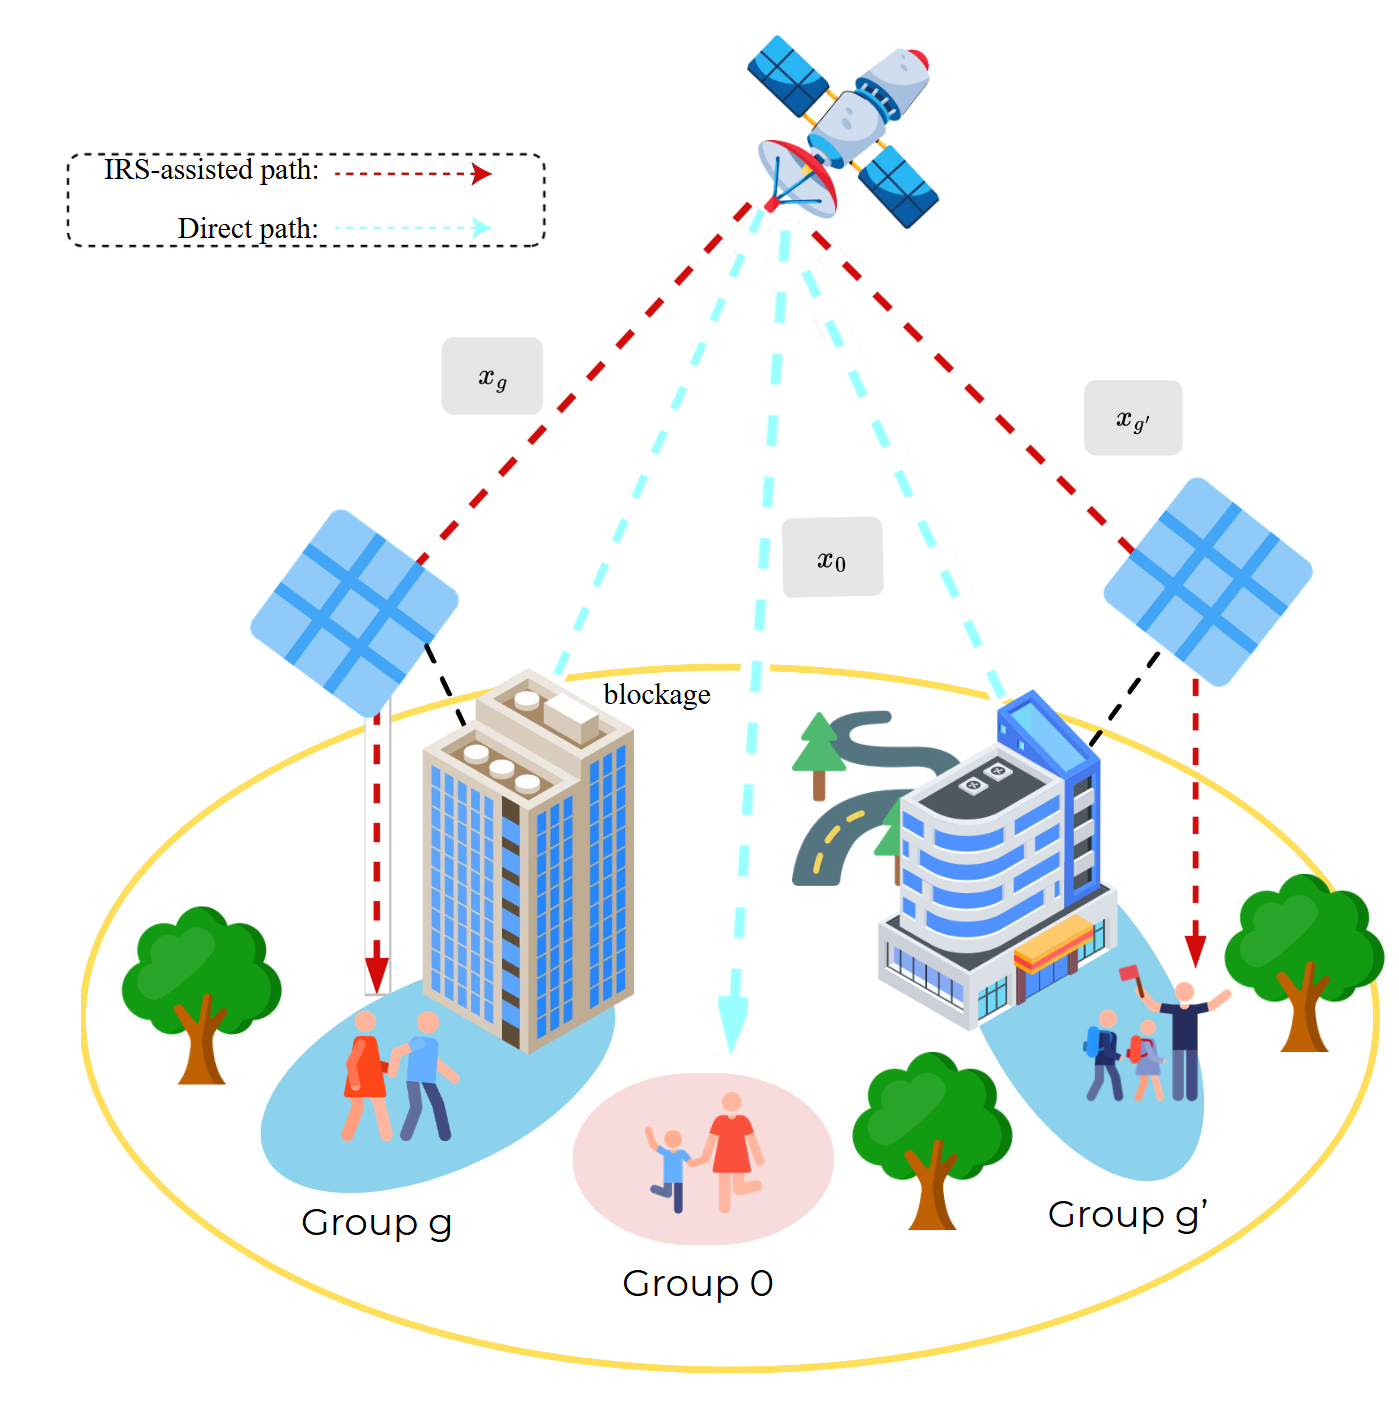
\includegraphics[width=0.65\linewidth]{images/ISTN_Comms}
    \caption{Proposed IRS-assisted grouped RSMA system in an ISTN downlink.
    The satellite simultaneously serves $G+1$ groups: Group~$0$ users with unobstructed satellite links receive the direct signal $x_0$, while Group~$g$ and Group~$g'$ users blocked by buildings are served via dedicated IRS panels carrying reflected signals $x_g$ and $x_{g'}$.
    Each IRS serves its assigned group through the phase-shift configuration $\boldsymbol{\Phi}_m$, chosen so that its reflected contributions combine coherently at those users.}
    \label{fig:istn_system}
\end{figure}

Operating such a network requires four coupled decisions at every scheduling interval,
namely the assignment of users to surfaces, the phase configuration of each surface, the
division of the transmit budget and the apportionment of the group common rate. Together they form a
mixed-integer non-convex problem admitting no tractable closed form, for which the
established remedy is to decompose the problem and alternate between the resulting
subproblems~\cite{luo2008dynamic,luo2010semidefinite}. That remedy is priced per channel realization, the solver retaining nothing between
invocations, so that every realization pays the iterative cost anew and a link whose
geometry follows user mobility pays it at the rate at which that geometry
changes~\cite{meng2023sum}.

Reinforcement learning inverts the arrangement. A policy trained once maps an observed
state directly onto an allocation, discharging the optimization burden offline and
answering each realization with a single forward
pass~\cite{sutton2018reinforcement,sun2018learning}. The four variables are not
independent but form a strict sequential dependency, the assignment fixing the grouping
that governs the phase design, the phase design shaping the effective channels that enter
the power allocation, and the resulting budget delimiting the feasible common-rate split.
That ordering motivates a hierarchical actor-critic
decomposition~\cite{levy2019learning,gong2023hierarchical}, a high-level actor committing
to the discrete assignment while dedicated low-level actors resolve the remainder in
sequence. The discrete complexity concentrates in the assignment, the number of feasible
user-to-surface associations growing exponentially in the user population. A variational
quantum circuit (VQC) represents a distribution over that space with a compact set of
trainable parameters~\cite{jerbi2021parametrized}, and because its input would otherwise
scale with both the user population and the panel count and so exceed a near-term
register~\cite{preskill2018quantum}, an autoencoder~\cite{hinton2006reducing} learns the
latent embedding on which the assignment actually depends,
following~\cite{nagy2025hybrid}.

\begin{table*}[t]
\centering
\caption{Comparison of existing works on IRS/RIS-assisted communication systems}
\label{tab:comparison_existing_works}
\setlength{\tabcolsep}{4pt}
\resizebox{\textwidth}{!}{%
\begin{tabular}{c|c|c|c|c|c|c|c|c|c|c|c}
\hline
\textbf{Ref.} 
& \textbf{Access} 
& \textbf{Blockage}
& \textbf{CSI}
& \textbf{Prop. Path}
& \multicolumn{3}{c|}{\textbf{IRS/RIS}}
& \textbf{RL} 
& \textbf{QC} 
& \textbf{QoS}
& \textbf{Obj.} \\
\cline{6-8}
& 
& 
& 
& 
& \textbf{Scale}
& \textbf{Type}
& \textbf{Phase}
& 
& 
& 
& \\
\hline

2019 {\cite{wu2019intelligent}} 
& MU-BF 
& -- 
& Perf. 
& Multi 
& Single 
& Passive 
& Cont. 
& -- 
& -- 
& Constr.
& Min-power \\

2022 {\cite{cao2022robust}} 
& SDMA 
& \checkmark 
& Imperf. 
& Multi 
& Single 
& Passive 
& Cont. 
& -- 
& -- 
& --
& Sum-rate \\

2023 {\cite{dong2022intelligent}} 
& TDMA 
& \checkmark 
& Perf. 
& Multi 
& Single 
& Passive 
& Cont. 
& -- 
& -- 
& --
& WSR \\

2023 {\cite{meng2023sum}}
& RSMA
& --
& Perf.
& Multi
& Single
& STAR
& Cont.
& \checkmark
& --
& Constr.
& Sum-rate \\

2025 {\cite{asif2024transmissive}}
& H-NOMA 
& --
& Perf. 
& Single 
& Single 
& Passive 
& Cont. 
& -- 
& -- 
& Constr.
& TA-SR \\

2025 {\cite{peng2025robust}} 
& RSMA 
& -- 
& Imperf. 
& Multi 
& Single 
& Passive 
& Disc. 
& -- 
& -- 
& Constr.
& WSR \\

2025 {\cite{han2025weighted}} 
& RSMA 
& -- 
& Perf. 
& Single 
& Single 
& Passive 
& Disc. 
& -- 
& -- 
& Constr.
& WSR \\

2025 {\cite{lv2025weighted}} 
& MU-BF 
& -- 
& Perf. 
& Multi 
& Single 
& Passive 
& Cont. 
& -- 
& -- 
& --
& WSR \\

2025 {\cite{fu2025average}} 
& NOMA 
& -- 
& Perf. 
& Multi
& Single 
& Passive 
& Cont. 
& \checkmark
& -- 
& Penalty
& ASR \\

2025 {\cite{li2025sum}} 
& RSMA 
& \checkmark 
& Perf. 
& Single 
& Multi 
& Passive 
& Cont. 
& -- 
& -- 
& Constr.
& Sum-rate \\

2026 {\cite{he2026weighted}} 
& RSMA 
& -- 
& Imperf. 
& Multi 
& Multi 
& Passive 
& Cont. 
& -- 
& -- 
& Constr.
& WSR \\

2026 {\cite{zhang2026satellite}} 
& RSMA 
& -- 
& Imperf.
& Multi
& Single
& Active
& Cont.
& -- 
& -- 
& Constr.
& Sum-rate \\

2026 {\cite{tan2025flexible}} 
& RSMA 
& -- 
& Perf. 
& Single 
& Single 
& Passive 
& Cont. 
& -- 
& -- 
& Constr.
& Sum-rate \\

\textbf{Proposed} 
& G-RSMA
& \checkmark 
& Imperf. 
& Multi 
& Multi 
& Passive 
& Disc.
& \checkmark 
& \checkmark 
& Penalty
& Sum-rate \\
\hline
\end{tabular}}
\end{table*}

Table~\ref{tab:comparison_existing_works} places the setting against the prior art. The
entries differ in access scheme, panel count, phase resolution and CSI assumption, and the
configuration studied here sits at the demanding end of each. That a per-realization
solver adapts poorly to a changing environment is itself an established
argument~\cite{meng2023sum}. What the table does not record, for the model-based and the
learned entries alike, is what producing one allocation costs. That is the question this
paper takes up, and it is answered in units that do not depend on the machine the policy
runs on.

\subsection{Contributions}

The framework developed here addresses that gap from the standpoint of decision cost
rather than of achievable rate. It resolves the four variables with a single hierarchical
policy that is trained once and thereafter commits to an allocation in one forward pass,
and it places a variational quantum circuit at the head of the hierarchy, where the
discrete complexity is concentrated. The contributions are summarized as follows.

\begin{itemize}
    \item We formulate sum-rate maximization for a multi-IRS-assisted grouped RSMA downlink in ISTN, jointly optimizing IRS-user link assignment, phase-shift configuration, transmit power allocation and common-rate distribution as a sequential dependency chain, and balancing aggregate rate against per-user QoS under discrete phase quantization, building blockage and imperfect CSI.

    \item We propose the HQC-HAC framework, which exploits that dependency.
    A quantum actor built on a variational quantum circuit resolves the combinatorial IRS-user assignment at the high level, three classical actors resolve the phase, power and common-rate decisions in sequence, and entropy regularization with an annealing schedule sustains exploration across all levels.

    \item We adapt the AE-VQC pairing of~\cite{nagy2025hybrid} by structuring what the circuit receives.
    An affinity feature map removes the dependence on the reflecting-element count $N$, and a dual-branch autoencoder compresses the result into a latent whose two blocks load onto the user and IRS registers indexed by the readout observables, so the compression preserves the user--IRS structure.

    \item We evaluate two instantiations differing only in the assignment actor and report
    what a decision costs in units independent of the implementation. The quantum
    instantiation matches its classical counterpart to within the spread across training
    seeds while carrying substantially fewer inference parameters, and the invocation
    count of every learned policy is constant in the user population where that of the
    solver grows. Ablations attribute this to the compression rather than to the register
    size, the observable set or the entangling structure, placing the contribution in
    parameter efficiency and amortized inference rather than in achievable rate.
\end{itemize}

\section{Related Works}
\label{sec:related}

\subsection{IRS-Assisted Grouped RSMA for Sum-Rate Optimization in ISTNs}

The foundational framework for IRS-assisted wireless networks was established by Wu and Zhang~\cite{wu2019intelligent}, who demonstrated that jointly optimizing active transmit beamforming at the access point and passive phase shifts at the surface substantially reduces the transmit power required to serve a multiuser MISO downlink.

The broader body of work summarized in Table~\ref{tab:comparison_existing_works} leaves the same axes open.
Ten of the twelve entries deploy a single reflecting panel, so the reflected coverage cannot follow spatially dispersed user groups, the exceptions being~\cite{li2025sum,he2026weighted}.
Eight presume perfect CSI, robust designs being confined to~\cite{cao2022robust,peng2025robust,he2026weighted,zhang2026satellite}, and continuous phase control is near-universal, with quantization appearing only in~\cite{peng2025robust,han2025weighted}.
Learning-based optimization is rare, adopted in~\cite{meng2023sum,fu2025average}, and no entry employs a quantum policy representation.
Blockage enters the propagation model in only three cases~\cite{cao2022robust,dong2022intelligent,li2025sum}.

\iffull
Building upon this beamforming paradigm, Tan et al.~\cite{tan2025flexible} extended IRS-assisted transmission to satellite downlink communications by proposing a flexible grouped RSMA scheme for sum-rate maximization in ISTNs.
In their system, the $K$ ground users are dynamically partitioned into two disjoint groups based on real-time channel conditions and potential line-of-sight obstructions: group $\mathcal{K}_1$ users are exclusively served via the satellite-IRS-user reflected link, while group $\mathcal{K}_2$ users communicate through the direct satellite-user link.
The decodable common rate within each group is thereby bounded by the weakest member of that subgroup rather than by the globally worst-performing user, which substantially alleviates the worst-user bottleneck inherent in flat RSMA designs.
Their joint problem spans satellite precoding beamforming, IRS phase-shift configuration, rate-splitting allocation and binary group selection, and was decomposed into four subproblems solved respectively by SDR with polyblock outer approximation, Riemannian manifold conjugate gradient descent on the phase manifold, alternating optimization for rate allocation, and simulated annealing for the binary assignment, the joint solution being recovered iteratively.

Despite reporting approximately 29\% sum-rate gain over the IRS-assisted RSMA baseline, the framework of~\cite{tan2025flexible} carries several limitations pertinent to realistic deployment.
The optimization presupposes perfect and instantaneous CSI at the satellite, whereas practical satellite links are susceptible to estimation errors arising from channel aging, Doppler effects, feedback delay, and limited feedback bandwidth.
Only a single IRS panel is considered, which is insufficient to extend reflected coverage across spatially dispersed user groups.
Furthermore, the iterative model-based solver must be re-run from scratch for every channel realization, and the framework provides no mechanism for adaptive policy adjustment under dynamic channel conditions or user mobility.
The proposed HQC-HAC framework addresses these deficiencies by optimizing IRS-user link assignment across multiple IRS panels under imperfect CSI, building blockage, and dynamic user mobility, replacing model-based sub-problem decomposition with a hierarchical reinforcement learning approach whose variational quantum policy representation manages the combinatorial complexity of multi-IRS user assignment.
\else
Building on that paradigm, Tan et al.~\cite{tan2025flexible} extended IRS-assisted
transmission to satellite downlinks with a flexible grouped RSMA scheme, partitioning the
$K$ users into a reflected group and a direct group so that each group's common rate is
bounded by its own weakest member rather than by the globally worst user. Their joint
problem over precoding, phase configuration, rate splitting and binary group selection is
decomposed into four subproblems and solved iteratively, reporting approximately $29\%$
sum-rate gain over an IRS-assisted RSMA baseline. Three limitations bear on deployment.
The design presupposes perfect instantaneous CSI, whereas practical satellite links suffer
estimation error from channel aging, Doppler and feedback delay; it admits a single panel
and therefore cannot extend reflected coverage across spatially dispersed groups; and its
model-based solver must be re-run from scratch at every channel realization, offering no
mechanism for adaptation under mobility. HQC-HAC addresses all three.
\fi

\subsection{Entropy-Regularized Hierarchical Reinforcement Learning and Hybrid Quantum-Classical Policies}

Hierarchical actor-critic (HAC) methods decompose complex decision problems into multiple levels of abstraction, with high-level actors committing to sub-goals that low-level actors subsequently fulfill~\cite{levy2019learning, bacon2017option}.
This temporal and functional decomposition has been demonstrated to accelerate learning in environments with large composite action spaces, including IRS-assisted wireless resource management, where jointly optimizing discrete and continuous variables over extended interaction horizons is otherwise costly to learn directly~\cite{gong2023hierarchical}.
Entropy regularization sustains policy diversity during training, the maximum-entropy objective of soft actor-critic~\cite{haarnoja2018soft} penalizing premature collapse to a deterministic policy.

Hybrid quantum-classical reinforcement learning extends this paradigm by replacing or augmenting classical policy networks with variational quantum circuits
(VQCs)~\cite{jerbi2021parametrized,kruse2023variational}.
VQCs model nonlinear policy mappings through parameterized quantum state transformations with comparatively compact trainable representations, which motivates their study for high-dimensional combinatorial
decisions and has prompted direct parameter-based comparisons against neural
networks~\cite{kolle2025evaluating}.
However, directly encoding high-dimensional wireless system states into a quantum register is impractical given current hardware constraints~\cite{preskill2018quantum}.
Nagy et al.~\cite{nagy2025hybrid} addressed this by jointly training an autoencoder (AE) with a VQC-based policy, where the AE compresses the original observation into a low-dimensional latent space suitable for quantum encoding.
This work embeds an AE-VQC actor within an entropy-regularized HAC structure.

\section{System Model and Problem Formulation}
\label{sec:model}

\subsection{Network and Association Model}

\iffull
\begin{table*}[t]
\centering
\caption{Summary of Main Notations}
\label{tab:variables}
\renewcommand{\arraystretch}{1.18}
\small
\singlespacing
\begin{tabularx}{\textwidth}{
>{\centering\arraybackslash}p{1.6cm}
>{\raggedright\arraybackslash}X
>{\centering\arraybackslash}p{1.6cm}
>{\raggedright\arraybackslash}X
}
\toprule
\textbf{Symbol} & \textbf{Description} 
& \textbf{Symbol} & \textbf{Description} \\
\midrule

$\mathcal{K}$ 
& Set of ground users
& $\mathcal{M}$ 
& Set of IRSs \\

$K$ 
& Number of ground users
& $M$ 
& Number of IRSs \\

$\mathcal{N}$ 
& Set of IRS reflecting elements
& $N$ 
& Number of reflecting elements \\

$\varphi_k$ 
& IRS-selection variable of user $k$
& $\mathcal{G}$ 
& Set of active transmission groups \\

$\mathcal{K}_g$ 
& Set of users assigned to group $g$
& $P_S$ 
& Maximum transmit power of the satellite \\

$s_k$ 
& Original message intended for user $k$
& $s_{c,g}$ 
& Common stream of group $g$ \\

$s_{k,p,g}$
& Private stream of user $k$ in group $g$
& $\boldsymbol{\Phi}_m$
& Phase-shift matrix of IRS $m$ \\

$w_{c,g}$
& Scalar precoding coefficient for $s_{c,g}$
& $w_{k,p,g}$
& Scalar precoding coefficient for $s_{k,p,g}$ \\

$\mathbf{w}$ 
& Set of scalar precoding coefficients
& $h$ 
& Effective channel coefficient \\

$\theta_{m,n}$ 
& Phase shift of the $n$-th IRS element
& $\mathcal{Q}_{\theta}$ 
& Quantized phase-angle set \\

$B$ 
& Number of phase quantization bits
& $g^{SU}\!,g^{SR}\!,g^{RU}$ 
& True channel coefficients of each link \\

$\hat{g}$ 
& Estimated channel coefficient
& $\Delta g$ 
& CSI estimation error \\

$x$ 
& Transmitted signal at the satellite
& $y_k$ 
& Received signal at user $k$ \\

$n_0$ 
& Additive white Gaussian noise
& $\sigma^2$ 
& Noise variance \\

$\gamma$ 
& SINR for decoding the corresponding stream
& $R_{k,c,g}$ 
& Common-stream decoding rate of user $k$ \\

$R_{c,g}$ 
& Decodable common rate of group $g$
& $C_{k,g}$ 
& Allocated common rate for user $k$ \\

$R_{k,p,g}$
& Achievable private rate of user $k$ in group $g$
& $\epsilon^{SU}\!,\epsilon^{SR}\!,\epsilon^{RU}$
& Rain-attenuation coefficient of each link \\

$R_k$ 
& Total achievable rate of user $k$
& $R_{\mathrm{tot}}$ 
& Achievable system sum-rate \\

$R_k^{\min}$ 
& Minimum QoS requirement of user $k$
& $\epsilon_{\mathrm{o}}$
& Outage level of the QoS chance constraint \\

$\gamma_{\mathrm d}$
& RL discount factor
& $\lambda_{\mathrm{GAE}}$
& GAE bias--variance parameter \\

$\epsilon_{\mathrm c}$
& PPO clipping range
& $\epsilon_{\mathrm q}$
& QoS-penalty guard constant \\

$\lambda_{D}$
& QoS-penalty weight
& $\beta$
& Entropy regularization coefficient \\

$\alpha_{AE}$
& Autoencoder loss weight
& $G_t$
& GAE $\lambda$-return regression target \\

$\rho_t$
& PPO importance-sampling ratio
& $\hat{A}_t$
& Generalized advantage estimate \\

$V(\cdot)$
& State-value function (critic)
& $\boldsymbol{\eta}$
& VQC trainable parameters \\

$c_{\mathrm s}$
& SPSA perturbation step
& $\tau$
& SoftmaxPQC inverse temperature (policy layer) \\

$\mathbf{s}_t$
& State: affinity feature vector
& $\mathbf{a}_t$
& Action $(\boldsymbol{\varphi},\boldsymbol{\Phi},\mathbf{w},\mathbf{C})$ \\

$\mathbf{z}_t$
& AE latent vector ($\in\mathbb{R}^{2n_q}$)
& $\bar{\mathbf{s}}_t$
& Group-normalized affinity state \\

$a_{k,m}$
& IRS path quality of user $k$ via IRS $m$
& $q_m$
& Mean affinity of IRS $m$ over users \\

$p_m$
& Received satellite-to-IRS power
& $\hat{\mathbf{s}}_t$
& AE reconstruction of $\mathbf{s}_t$ \\

$\mathcal{U}$, $\mathcal{R}$
& User-qubit and IRS-qubit index sets
& $\mathbf{W}_{\mathrm{proj}}$
& AE user-branch projection matrix \\

$\mathcal{L}_{AE}$
& AE reconstruction loss
&
& \\

$n_q$
& Number of qubits
& $L$
& Number of VQC variational layers \\

$\hat{\mathbf{o}}_t$
& VQC measurement (readout) vector
& $N_Q$
& Number of readout observables \\

$\boldsymbol{\lambda}_y, \boldsymbol{\lambda}_z$
& Trainable encoding scales
& $\boldsymbol{\gamma}, \mathbf{b}_{\mathrm{LN}}$
& Encoding LayerNorm learnable affine \\

$\kappa$
& CSI error coefficient
& $\varepsilon$
& CSI error variable, $\varepsilon\sim\mathcal{CN}(0,1)$ \\

$\varsigma_k$
& Rate shortfall of user $k$
& $R_{\mathrm{LoS}}$
& Satellite line-of-sight ground radius \\

$\boldsymbol{\theta}$
& VQC variational angles (component of $\boldsymbol{\eta}$)
& $\mathbf{w}_p,\mathbf{w}_c$
& Private and common power vectors \\

$S_{\mathrm{tr}}$
& Measurement shots during training
& $S_{\mathrm{ev}}$
& Measurement shots at inference \\

$\epsilon_{\mathrm{LN}}$
& LayerNorm numerical-stability constant
& $\boldsymbol{\gamma},\mathbf{b}_{\mathrm{LN}}$
& Encoding LayerNorm learnable affine \\

$\beta_{\mathrm{blk}}$
& Blocking factor on the direct link
& $\Omega_{sf}$
& Average shadow-fading power gain \\
\end{tabularx}
\end{table*}
\fi


We consider an IRS-assisted grouped rate-splitting multiple access (RSMA) downlink communication system in an integrated satellite-terrestrial network (ISTN). 
In the considered system, a satellite serves a set of ground users with the assistance of intelligent reflecting surfaces (IRSs), which are deployed on high buildings to enhance the wireless propagation environment and support users experiencing weak or blocked direct satellite-to-user links. 
The satellite is assumed to act as the central controller, which determines the transmission strategy, resource allocation, and IRS-assisted communication mode according to the observed channel conditions and user requirements.

Let $\mathcal{K}=\{1,2,\ldots,K\}$ denote the set of downlink ground users, where $K$ is the total number of users. 
The satellite transmits one independent message to each user, the message intended for
user $k \in \mathcal{K}$ being denoted by $s_k$, so that the scheduled message set is
$s=\{s_1,\ldots,s_K\}$.

We consider $M$ IRSs deployed on the rooftops of buildings to assist the satellite downlink transmission. 
Let $\mathcal{M}=\{1,2,\ldots,M\}$ denote the set of IRSs. 
Each IRS is equipped with $N$ passive reflecting elements, which can independently adjust the phase shift of the incident signal. 
The IRSs are assumed to be connected to the central controller, and their reflection coefficients are configured according to the channel conditions and user association decisions. For IRS $m \in \mathcal{M}$, the reflection matrix is defined as
\begin{equation}
    \boldsymbol{\Phi}_m
    =
    \operatorname{diag}
    \left(
    e^{j\theta_{m,1}},
    e^{j\theta_{m,2}},
    \ldots,
    e^{j\theta_{m,N}}
    \right),
\end{equation}
where $\theta_{m,n}$ denotes the phase shift of the $n$-th reflecting element at IRS $m$. Practical surfaces resolve the phase only to a finite number of levels, so with $B$
quantization bits each element selects its shift from the uniformly spaced
set~\cite{peng2025robust,han2025weighted}
\begin{equation}
    \mathcal{Q}_{\theta}
    =
    \left\{\left. \theta^{(q)} = \frac{2\pi q}{2^{B}} \;\right|\;
    q = 0,1,\ldots,2^{B}-1 \right\}.
\end{equation}

To determine the transmission mode of each user, we define an IRS-selection variable for every user $k \in \mathcal{K}$. 
Since the considered system includes $M$ IRSs, each user can either be served through the direct satellite-to-user link or through one of the IRS-assisted reflected links. 
Therefore, the IRS-selection variable $\varphi_k \in \{0,1,\ldots,M\}$ is defined for every
$k \in \mathcal{K}$ as
\begin{equation}
    \varphi_k =
    \begin{cases}
        0, & \text{user } k \text{ served by the direct link},\\
        m, & \text{user } k \text{ served by IRS } m.
    \end{cases}
\end{equation}

\subsection{Channel Model}

Due to the long propagation distance between the satellite and ground nodes, the satellite-to-user (SU) and satellite-to-IRS (SR) links are dominated by large-scale path loss and rain attenuation following the ITU-R model~\cite{itu618}.
The IRS-to-user (RU) link additionally exhibits small-scale Rayleigh fading and distance-dependent path loss~\cite{3gpp38811}.
The true channel coefficients of the three links are modeled as
\begin{equation}
\begin{aligned}
    g^{SU}_k
    &=
    \frac{c\sqrt{G_S G_U \epsilon^{SU}_k}}{4\pi f_{SU} d^{SU}_k},
    \\[2mm]
    g^{SR}_{m}
    &=
    \frac{c\sqrt{G_S \epsilon^{SR}_{m}}}{4\pi f_{SR} d^{SR}_{m}},
    \\[2mm]
    g^{RU}_{m,k}
    &=
    \sqrt{
        G_U \cdot \Omega_{sf}
        \cdot
        \!\left(\frac{d_0}{d^{RU}_{m,k}}\right)^{\!\alpha}
        \cdot\,
        \epsilon^{RU}_{m,k}
    }
    \;\tilde{g}^{sf}_{m,k},
\end{aligned}
\end{equation}
for every $m \in \mathcal{M}$ and $k \in \mathcal{K}$, where $c$ is the speed of light; $G_S$ and $G_U$ are the satellite transmit and user receive antenna gains; $f_{SU}$ and $f_{SR}$ are the corresponding carrier frequencies; $d^{SU}_k$, $d^{SR}_{m}$, and $d^{RU}_{m,k}$ denote the satellite-to-user, satellite-to-IRS, and IRS-to-user link distances; $\epsilon^{SU}_k$, $\epsilon^{SR}_{m}$, and $\epsilon^{RU}_{m,k}$ are the rain-attenuation coefficients modeled as lognormal random variables per the ITU-R standard; $\Omega_{sf}$ is the average shadow-fading power gain of the IRS-to-user link; $\alpha$ is the path-loss exponent; $d_0$ is the reference distance; and $\tilde{g}^{sf}_{m,k} \sim \mathcal{CN}(0,1)$ represents the small-scale Rayleigh fading component.
When the satellite-to-user line of sight is intersected by a building, the affected coefficient $g^{SU}_k$ is scaled by a blocking factor $\beta_{\mathrm{blk}} \in (0,1]$, so that a blocked user retains a weak direct path rather than losing it entirely.
Each channel coefficient is complex, with a random propagation phase uniformly distributed on $[0, 2\pi)$, which is tracked via Doppler compensation at the satellite.

Since the satellite acquires only an imperfect estimate of each channel coefficient, the estimated channel $\hat{g}$ and the true channel $g$ are related by a multiplicative error model:
\begin{equation}
    \hat{g} = g + \Delta g,
    \qquad
    \Delta g = \kappa \lvert g \rvert \varepsilon,
    \qquad
    \varepsilon \sim \mathcal{CN}(0,1),
\end{equation}
where $\kappa \geq 0$ is the relative error coefficient applied uniformly to all three links.
This yields the estimated channels $\hat{g}^{SU}_k$, $\hat{g}^{SR}_{m}$, and $\hat{g}^{RU}_{m,k}$, which are used for all precoding and resource allocation design.
The policy is designed on the estimated channels alone, the assignment actor consuming per-user path qualities and the phase actor the estimated cascaded coefficients, whereas the environment scores the achieved rate on the true channels $g$.

\subsection{Transmission and Decoding}

Following the RSMA principle~\cite{mao2018rate}, each user message $s_k$ of user $k \in \mathcal{K}_g$ is split into a common sub-message $s_{c,g}$ and a private sub-message $s_{k,p,g}$.
However, not all IRSs are necessarily selected by the agent at each decision step. 
Therefore, the number of active groups is denoted by $G$, where $G \leq M+1$.
We define the set of scheduled user messages after splitting as

\[
\tilde{\mathbf{s}} = [\,s_{c,1}, s_{c,2}, \ldots, s_{c,G},\; \{s_{k,p,g}\}_{g \in \mathcal{G},\, k \in \mathcal{K}_g}\,].
\]

A single-antenna satellite precludes spatial beamforming, so each stream carries a
scalar coefficient, $w_{c,g} \in \mathbb{C}$ for the common stream of group $g$ and
$w_{k,p,g} \in \mathbb{C}$ for the private stream of user $k \in \mathcal{K}_g$, and the
transmitted signal is
\begin{equation}
    x
    =
    \sum_{g \in \mathcal{G}} w_{c,g}s_{c,g}
    +
    \sum_{g \in \mathcal{G}}\sum_{k \in \mathcal{K}_g} w_{k,p,g}s_{k,p,g},
\end{equation}
where $s_{c,g}$ is the common stream intended for all users in group $\mathcal{K}_g$, and $s_{k,p,g}$ is the private stream intended only for user $k$ in group $g$.
The scalar precoding coefficients are constrained by the maximum transmit power of the satellite, i.e.,
$\sum_{g \in \mathcal{G}} |w_{c,g}|^2 + \sum_{g \in \mathcal{G}}\sum_{k \in \mathcal{K}_g} |w_{k,p,g}|^2 \leq P_S$,
where $P_S$ denotes the maximum transmit power of the satellite.



After receiving $y_k$, each user decodes its group-specific common stream and then its
private stream by successive interference cancellation, following the standard RSMA
decoding order~\cite{mao2018rate,mao2022rate}.
For user $k \in \mathcal{K}_g$, the SINRs for decoding the common stream $s_{c,g}$ and the private stream $s_{k,p,g}$ are respectively given by
\begin{equation}
\begin{aligned}
    \gamma_{k,c,g}
    &=
    \frac{
        |h_k w_{c,g}|^2
    }{
        \sum_{g' \neq g}
        |h_k w_{c,g'}|^2
        \!+\!
        \sum_{g' \in \mathcal{G}}\!\sum_{j \in \mathcal{K}_{g'}}\!
        |h_k w_{j,p,g'}|^2
        \!+\!
        \sigma^2
    },
    \\[2mm]
    \gamma_{k,p,g}
    &=
    \frac{
        |h_k w_{k,p,g}|^2
    }{
        \sum_{g' \in \mathcal{G}}\!\sum_{\substack{j \in \mathcal{K}_{g'} \\ j \neq k}}\!
        |h_k w_{j,p,g'}|^2
        \!+\!
        \sum_{g' \neq g}
        |h_k w_{c,g'}|^2
        \!+\!
        \sigma^2
    }.
\end{aligned}
\end{equation}
Since the common stream $s_{c,g}$ is intended for all users in group $\mathcal{K}_g$, it must be successfully decoded by every user in that group. 
Therefore, the achievable common rate of group $g$ is limited by the user with the lowest common-stream decoding rate. 
For user $k \in \mathcal{K}_g$, the common-stream decoding rate and the resulting group common rate are given by
\begin{equation}
    R_{k,c,g}
    =
    \log_2\left(1 + \gamma_{k,c,g}\right),
    \qquad
    R_{c,g}
    =
    \min_{k \in \mathcal{K}_g} R_{k,c,g}.
\end{equation}

Let $C_{k,g}$ denote the portion of the group common rate allocated to user $k \in \mathcal{K}_g$. 
The common-rate allocation must satisfy
\begin{equation}
    \sum_{k \in \mathcal{K}_g} C_{k,g}
    =
    R_{c,g},
    \quad
    C_{k,g} \geq 0.
\end{equation}

After decoding and removing the common stream, user $k$ decodes its private stream, achieving rate $R_{k,p,g} = \log_2(1 + \gamma_{k,p,g})$.
The total achievable rate of user $k$ is thus $R_k = R_{k,p,g} + C_{k,g}$, and the system sum-rate is
\begin{equation}
    R_{\mathrm{tot}}
    =
    \sum_{k \in \mathcal{K}}
    R_k
    =
    \sum_{g \in \mathcal{G}} R_{c,g}
    +
    \sum_{g \in \mathcal{G}}\sum_{k \in \mathcal{K}_g} R_{k,p,g}.
\end{equation}

\subsection{Optimization Problem}

The objective is to maximize the system sum-rate by jointly optimizing the IRS-selection variables, the scalar precoding coefficients, the IRS phase-shift matrices, and the common-rate allocation.
Specifically, the optimization variables are given by
$\boldsymbol{\varphi}=\{\varphi_k\}_{k\in\mathcal{K}}$, 
$\mathbf{w}=\{w_{c,g},w_{k,p,g}\}_{g\in\mathcal{G},k\in\mathcal{K}_g}$,
$\boldsymbol{\Phi}=\{\boldsymbol{\Phi}_m\}_{m\in\mathcal{M}}$, 
and $\mathbf{C}=\{C_{k,g}\}_{k\in\mathcal{K}_g,g\in\mathcal{G}}$. 
The sum-rate maximization problem is formulated as
\begin{subequations}\label{eq:P0}
\begin{align}
    \text{(P0):} \quad
    \max_{\boldsymbol{\varphi},\mathbf{w},\boldsymbol{\Phi},\mathbf{C}}
    \quad
    &
    R_{\mathrm{tot}}
    \label{eq:P0_objective}
    \\
    \text{s.t.}\;
    &
    \varphi_k \in \{0,1,\ldots,M\},
    \quad \forall k \in \mathcal{K},
    \label{eq:P0_selection}
    \\[1mm]
    &
    \sum_{g \in \mathcal{G}} |w_{c,g}|^2
    +
    \sum_{g \in \mathcal{G}}\sum_{k \in \mathcal{K}_g} |w_{k,p,g}|^2
    \leq P_S,
    \label{eq:P0_power}
    \\[1mm]
    &
    \theta_{m,n} \in \mathcal{Q}_{\theta},
    \quad \forall m \in \mathcal{M}, \forall n \in \mathcal{N},
    \label{eq:P0_phase}
    \\[1mm]
    &
    \boldsymbol{\Phi}_m
    =
    \operatorname{diag}
    \bigl(
    e^{j\theta_{m,1}},
    \ldots,
    e^{j\theta_{m,N}}
    \bigr),
    \ \forall m,
    \label{eq:P0_phi}
    \\[1mm]
    &
    \sum_{k \in \mathcal{K}_g} C_{k,g}
    = R_{c,g},
    \quad \forall g \in \mathcal{G},
    \label{eq:P0_common_rate}
    \\[1mm]
    &
    C_{k,g} \geq 0,
    \quad \forall k \in \mathcal{K}_g,\ \forall g \in \mathcal{G},
    \label{eq:P0_nonnegative}
    \\[1mm]
    &
    \Pr\{ R_k \geq R_k^{\min} \mid \hat{g} \} \geq 1-\epsilon_{\mathrm{o}},
    \ \forall k.
    \label{eq:P0_qos}
\end{align}
\end{subequations}

In the above problem (P0),~\eqref{eq:P0_selection} limits the values of the IRS-selection variables, which determine whether each user is served through the direct satellite-to-user link or one of the available IRS-assisted links.
This choice also induces the grouping, so that $\mathcal{K}_g$ and $G$ in the remaining constraints are themselves functions of $\boldsymbol{\varphi}$.~\eqref{eq:P0_power} guarantees that the total transmit power of the satellite does not exceed the maximum power budget.~\eqref{eq:P0_phase} restricts the phase shift of each IRS reflecting element to the discrete quantized phase-angle set, while constraint~\eqref{eq:P0_phi} defines the corresponding passive IRS phase-shift matrix. 
Constraint~\eqref{eq:P0_common_rate} requires that the allocated common rates fully exhaust the group common rate, i.e., the entire decodable common rate of each group is distributed among its members with no waste.
Constraint~\eqref{eq:P0_nonnegative} ensures non-negativity of the allocated common rates, and constraint~\eqref{eq:P0_qos}~\cite{wang2014outage,nemirovski2007convex} imposes the per-user minimum-rate requirement at an outage level $\epsilon_{\mathrm{o}}$.
\section{Proposed HQC-HAC Framework}
\label{sec:framework}

\subsection{Overall Framework}
\begin{figure}[t]
    \centering
    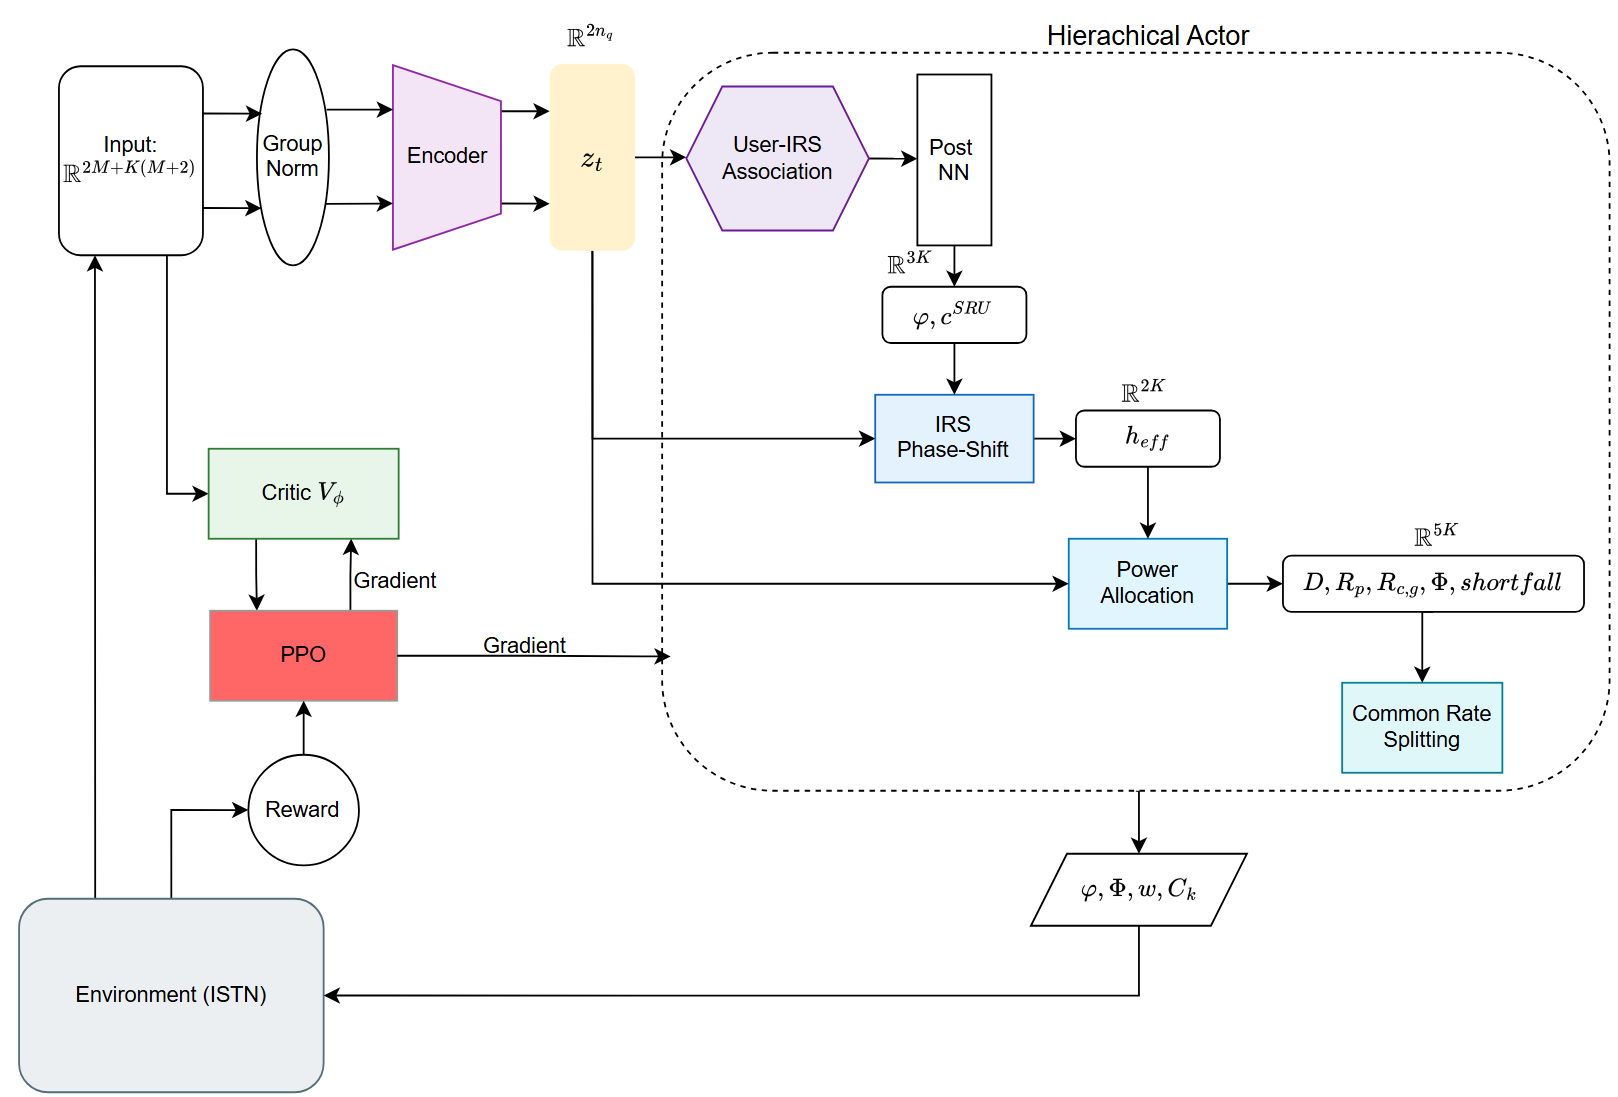
\includegraphics[width=\linewidth]{images/HQC-HAC}
    \caption{Overall HQC-HAC hierarchical actor-critic framework. The quantum actor (top level) resolves the discrete IRS-user assignment $\boldsymbol{\varphi}$ via a VQC, while three sequential classical sub-actors (Phase MLP, Power MLP, and Common-Rate MLP) optimize the remaining continuous variables conditioned on the chosen assignment. A shared classical critic provides state-value estimates for computing advantages across all actors.}
    \label{fig:framework}
\end{figure}

\iffull
Problem~(P0) is a mixed-integer non-convex program. 
The assignment $\boldsymbol{\varphi}$ is discrete over a set of size $(M+1)^K$, the per-element phase shifts are confined to the quantized set $\mathcal{Q}_\theta$, and both couple to the continuous powers $\mathbf{w}$ and common-rate shares $\mathbf{C}$ through the SINR expressions, which also render $R_{\mathrm{tot}}$ non-concave.
The problem is therefore NP-hard in general~\cite{luo2008dynamic}, and the model-based relaxations discussed in Section~\ref{sec:related}, such as semidefinite relaxation~\cite{luo2010semidefinite} and alternating optimization, carry the limitations set out there. 
We instead learn a policy that maps the observed state directly to the joint action.

The four decision variables exhibit a strict sequential dependency: the assignment $\boldsymbol{\varphi}$ fixes which IRS panels are active, and thereby the number of active groups $G$ and the dimension of the common-power vector $\mathbf{w}_c$; the active set governs the effective channels that underpin the phase-shift design $\boldsymbol{\Phi}$; the resulting channel gains shape the power-allocation landscape $(\mathbf{w}_p,\mathbf{w}_c)$; and the allocated powers delimit the feasible common-rate split $\mathbf{C}$.
We adopt a hierarchical actor--critic decomposition that mirrors this ordering: a high-level actor commits to the discrete assignment, and three low-level actors resolve the continuous variables in sequence, each conditioned on the decisions made upstream.

The high-level assignment remains the principal source of difficulty, since $\{0,1,\ldots,M\}^K$ is non-differentiable and grows exponentially in both $K$ and $M$. 
We therefore place a variational quantum circuit (VQC) at the top of the hierarchy, where an $n_q$-qubit state parameterizes a distribution over this space compactly.
Once $\boldsymbol{\varphi}$ is fixed the remaining sub-problems are smooth, continuous, and low-dimensional, and are handled by classical multi-layer perceptrons (MLPs); reserving the quantum circuit for the combinatorial bottleneck is what renders the framework \emph{hybrid} quantum--classical.





At each decision step~$t$ the raw channel observation is condensed into the affinity state $\mathbf{s}_t$, which both the quantum actor and the shared critic consume, and an autoencoder further compresses it to the latent $\mathbf{z}_t\in\mathbb{R}^{2n_q}$ that the $n_q$-qubit register encodes (Section~\ref{sec:ae}). Following the data flow in Fig.~\ref{fig:framework}, the VQC maps $\mathbf{z}_t$ to a measurement vector, which the quantum actor's policy layer converts into a categorical distribution over candidate assignments; sampling it yields $\boldsymbol{\varphi}$. The three sub-actors then act in sequence: the Phase MLP produces the quantized phase indices $\boldsymbol{\theta}_{\mathrm{idx}}$ and hence $\boldsymbol{\Phi}$, the Power MLP allocates the private and common powers $(\mathbf{w}_p,\mathbf{w}_c)$, and the Common-Rate MLP distributes the group common rates $\mathbf{C}$ among users. The joint action is applied to the environment, which returns the next state and the reward of~\eqref{eq:reward}.

All four actors and the shared critic are trained together by proximal policy optimization (PPO)~\cite{schulman2017proximal} with entropy regularization annealed over training. Sections~\ref{sec:ae}--\ref{sec:training} describe the autoencoder, the quantum circuit, and the training procedure in detail.
\else
Problem (P0) is a mixed-integer non-convex program~\cite{luo2008dynamic,luo2010semidefinite}
whose four variables are not independent. The assignment fixes which users share a group,
the grouping conditions the phase design, the resulting effective channels shape the power
allocation, and the power budget delimits the feasible common-rate split. HQC-HAC follows
that order. At each step the raw channel observation is condensed into the affinity state
$\mathbf{s}_t$ of~\eqref{eq:affinity}, an autoencoder compresses it to a latent
$\mathbf{z}_t$, and a variational quantum circuit reading that latent emits the assignment,
which is the only genuinely combinatorial variable since
$\{0,1,\ldots,M\}^K$ is non-enumerable at the scales considered. Three classical sub-actors
then resolve phase, power and common rate in sequence, as shown in
Fig.~\ref{fig:framework}. All four actors and a shared critic are trained together by
proximal policy optimization~\cite{schulman2017proximal}.
\fi

\subsection{Autoencoder-Based Latent State Representation}
\label{sec:ae}
\iffull
Directly encoding the raw environment observation into a quantum register is impractical, since its dimension $M(3+2K+2N)+3K$ grows with the number of IRS elements $N$, which is unrelated to the IRS-user assignment decision.
The quantum actor instead operates on the compact \emph{affinity state} $\mathbf{s}_t \in \mathbb{R}^{K(M+2)+2M}$ of Section~\ref{sec:framework}, which retains only the information pertinent to link assignment.
Even so, $\mathbf{s}_t$ still exceeds the register, requiring one qubit per two components.
The compression is therefore marginal at the smallest configuration, yet it is precisely what renders the larger ones representable. 
The affinity state is structured as
\begin{equation}
    \mathbf{s}_t
    =
    \bigl[
      a_{k,m}, \;
      R_k^{\min},\;
      |\hat{g}^{SU}_k|,\;
      q_m,\; p_m
    \bigr],
    \label{eq:affinity}
\end{equation}
where $a_{k,m} = |\hat{g}^{SR}_m| \sum_{n=1}^{N} |\hat{g}^{RU}_{m,n,k}|$ is the IRS path quality for user $k$ via IRS $m$, $q_m = \frac{1}{K}\sum_{k=1}^{K} a_{k,m}$ is the mean affinity of IRS $m$ across all users, and $p_m = |\hat{g}^{SR}_m|^2$ is the received satellite-IRS power.
The affinity, direct-link, and IRS blocks are standardized separately before encoding, yielding $\bar{\mathbf{s}}_t$.

A dual-branch encoder maps $\bar{\mathbf{s}}_t$ to the latent vector $\mathbf{z}_t \in \mathbb{R}^{2n_q}$, where $n_q$ is the number of qubits. As illustrated in Fig.~\ref{fig:ae_process}, the encoder comprises two parallel branches that process IRS-level and user-level information separately prior to concatenation. The \emph{IRS branch} maps the IRS summary statistics $[q_m, p_m]_{m=1}^{M} \in \mathbb{R}^{2M}$ through a two-layer MLP,
\begin{equation}
    \mathbf{z}^{\mathcal{R}}
    =
    \mathbf{W}_{2}^{\mathcal{R}}
    \,\mathrm{ReLU}\bigl(
      \mathbf{W}_{1}^{\mathcal{R}}[q_1,p_1,\ldots,q_M,p_M]^\top
      + \mathbf{b}_{1}^{\mathcal{R}}
    \bigr)
    + \mathbf{b}_{2}^{\mathcal{R}}
    \in \mathbb{R}^{2M},
\end{equation}
where $\mathbf{W}_{1}^{\mathcal{R}} \in \mathbb{R}^{16 \times 2M}$ and $\mathbf{W}_{2}^{\mathcal{R}} \in \mathbb{R}^{2M \times 16}$. The \emph{user branch} applies a shared two-layer micro-encoder independently to each user $k$, following the parameter-sharing scheme of set-encoding architectures~\cite{zaheer2017deep},
\begin{equation}
    \mathbf{z}_k
    =
    \mathbf{W}_{2}^{\mathcal{U}}
    \,\mathrm{ReLU}\bigl(
      \mathbf{W}_{1}^{\mathcal{U}}[a_{k,1},\ldots,a_{k,M},R_k^{\min},|\hat{g}^{SU}_k|]^\top
      + \mathbf{b}_{1}^{\mathcal{U}}
    \bigr)
    + \mathbf{b}_{2}^{\mathcal{U}}
    \in \mathbb{R}^{2},
    \quad \forall k \in \mathcal{K},
\end{equation}
where $\mathbf{W}_{1}^{\mathcal{U}} \in \mathbb{R}^{8 \times (M+2)}$ and $\mathbf{W}_{2}^{\mathcal{U}} \in \mathbb{R}^{2 \times 8}$ are shared across all $K$ users. A linear map $\mathbf{W}_{\mathrm{proj}} \in \mathbb{R}^{2(n_q-M) \times 2K}$ projects the $K$ stacked embeddings onto the user block, $\mathbf{z}^{\mathcal{U}} = \mathbf{W}_{\mathrm{proj}}[\mathbf{z}_1^\top,\ldots,\mathbf{z}_K^\top]^\top$, and the latent concatenates the two branches as $\mathbf{z}_t = [\mathbf{z}^{\mathcal{U}} \,\|\, \mathbf{z}^{\mathcal{R}}] \in \mathbb{R}^{2n_q}$, whose blocks are loaded onto the user qubits $\mathcal{U}$ and the IRS qubits $\mathcal{R}$ of Section~\ref{sec:vqc}.
Keeping the branches apart is what gives that mapping content.
Both the cross-block bridges and the user--IRS observables of Section~\ref{sec:vqc} are defined over this partition, so a single encoder that mixed the two sides would leave a user qubit and an IRS qubit holding arbitrary combinations, and observables meant to track the assignment would reduce to a generic set.
The separation also leaves the entangling gates as the only stage at which features from the two blocks are multiplied together.

\begin{figure}[t]
    \centering
    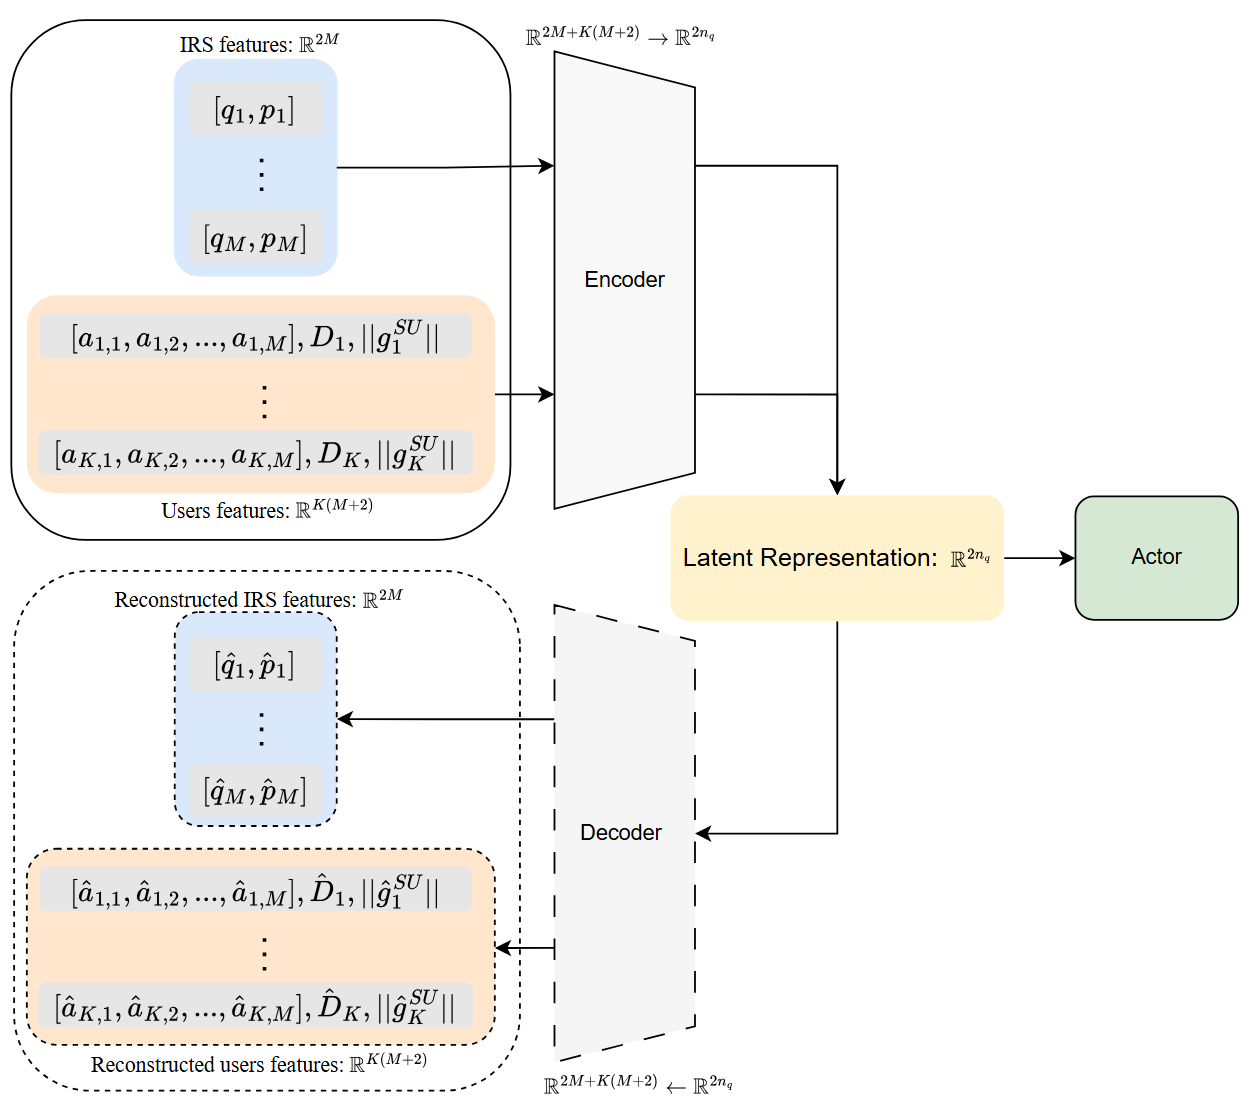
\includegraphics[width=0.72\linewidth]{images/AE_Process}
    \caption{Dual-branch autoencoder architecture for latent state compression.
    The encoder (top path) processes IRS summary features $[q_m, p_m]$ and per-user affinity features $[a_{k,m}, R_k^{\min}, |\hat{g}^{SU}_k|]$ through separate branches before concatenating into the latent representation $\mathbf{z}_t \in \mathbb{R}^{2n_q}$, which is forwarded to the quantum actor.
    The decoder (bottom path, active during training only) reconstructs the input feature vector $\hat{\mathbf{s}}_t$ from $\mathbf{z}_t$ and evaluates the reconstruction loss $\mathcal{L}_{AE} = \frac{1}{2}\|\hat{\mathbf{s}}_t - \bar{\mathbf{s}}_t\|^2$ to regularize the latent space.}
    \label{fig:ae_process}
\end{figure}

The decoder is a single stack rather than a mirror of the two-branch encoder. 
It expands $\mathbf{z}_t$ through rectified-linear hidden layers, after which a linear output layer returns the reconstruction $\hat{\mathbf{s}}_t$ to the width of $\mathbf{s}_t$, producing the reconstruction loss
\begin{equation}
    \mathcal{L}_{AE}
    =
    \frac{1}{2}
    \bigl\|\hat{\mathbf{s}}_t - \bar{\mathbf{s}}_t\bigr\|^2,
    \label{eq:ae_loss}
\end{equation}
where $\bar{\mathbf{s}}_t$ is the standardized affinity state. 
The decoder is used only during training and is discarded at inference, where only the encoder and the latent $\mathbf{z}_t$ are forwarded to the VQC.

The autoencoder is trained jointly and end-to-end with the rest of the framework, following the latent-observation approach of~\cite{nagy2025hybrid}. 
The reconstruction loss in~\eqref{eq:ae_loss} enters the policy objective as an auxiliary regularizer of weight $\alpha_{AE}$, so the encoder receives gradients from both $\mathcal{L}_{AE}$ and the reinforcement-learning loss back-propagated through the quantum actor.
The reconstruction term is retained throughout as a structural regularizer that preserves the informativeness of $\mathbf{z}_t$, with $\alpha_{AE}$ balancing representational fidelity against task performance.

Joint optimization is preceded by a short reconstruction-only \emph{warm-up} in which the autoencoder alone is updated and every other component is held fixed.
It is fitted on synthetic samples from the standardized input distribution rather than on environment rollouts, which suffices to condition the encoder so that the first policy gradients do not act upon an untrained representation.
\else
Encoding the raw observation into a quantum register is impractical, since angle encoding
would demand roughly one qubit per feature, that is $44$ qubits at Case~2 and $81$ at the
$K{=}15$ scale, placing state-vector simulation with per-step gradients out of reach. The
observation is therefore first reduced to an affinity state
\begin{equation}
    \mathbf{s}_t
    =
    \bigl[ a_{k,m}, \; R_k^{\min},\; |\hat{g}^{SU}_k|,\; q_m,\; p_m \bigr],
    \label{eq:affinity}
\end{equation}
which summarizes each user--IRS pair by a scalar path quality and each IRS by its mean
affinity and received power, so that the description no longer grows with the number of
reflecting elements. A dual-branch encoder then maps $\mathbf{s}_t$ to
$\mathbf{z}_t\in\mathbb{R}^{2n_q}$, one branch per IRS and one shared branch applied to
every user, the shared branch making the user block permutation-equivariant in the sense
of~\cite{zaheer2017deep}. The two blocks are loaded onto the IRS and user qubit registers
indexed by the readout observables, so the compression preserves the user--IRS structure
the assignment depends on rather than its dimension alone, following the hybrid pairing
of~\cite{nagy2025hybrid}. A decoder reconstructs the group-normalized state and is trained
by
\begin{equation}
    \mathcal{L}_{AE} = \frac{1}{2} \bigl\|\hat{\mathbf{s}}_t - \bar{\mathbf{s}}_t\bigr\|^2,
    \label{eq:ae_loss}
\end{equation}
jointly with the rest of the framework after a short reconstruction-only warm-up. The
decoder is discarded at inference, so it costs nothing at deployment. The register stays
at $n_q{=}8$ at both scales.
\fi

\subsection{Variational Quantum Circuit}
\label{sec:vqc}
\begin{figure}[t]
\centering
\resizebox{0.95\linewidth}{!}{%
\begin{quantikz}[row sep=0.4cm, column sep=0.45cm]
\lstick{$|0\rangle\,q_0$} & \gate{H}
  & \gate{R_y(\alpha_0)}\gategroup[4,steps=2,style={dashed,rounded corners,fill=purple!10},background]{$U_E(\mathbf{z};\boldsymbol{\lambda})$}
  & \gate{R_z(\delta_0)} &
  & \gate{R_y(\theta^{y}_0)}\gategroup[4,steps=2,style={dashed,rounded corners,fill=blue!10},background]{$U_L(\boldsymbol{\theta})$}
  & \gate{R_z(\theta^{z}_0)} &
  & \ctrl{1}\gategroup[4,steps=2,style={dashed,rounded corners,fill=orange!18},background]{$U_{\rm ent}$}
  & \ctrl{3}
  & \meter{}\gategroup[4,steps=1,style={dashed,rounded corners,fill=green!10},background]{$\hat{\mathbf{o}}_t$} \\
\lstick{$|0\rangle\,q_1$} & \gate{H}
  & \gate{R_y(\alpha_1)} & \gate{R_z(\delta_1)} &
  & \gate{R_y(\theta^{y}_1)} & \gate{R_z(\theta^{z}_1)} &
  & \control{} & \qw & \meter{} \\
\lstick{$\vdots$} & \setwiretype{n}\vdots & \vdots & \vdots & & \vdots & \vdots & & \vdots & \vdots & \\
\lstick{$|0\rangle\,q_{n_q-1}$} & \gate{H}
  & \gate{R_y(\alpha_{n_q-1})} & \gate{R_z(\delta_{n_q-1})} &
  & \gate{R_y(\theta^{y}_{n_q-1})} & \gate{R_z(\theta^{z}_{n_q-1})} &
  & \qw & \control{} & \meter{}
\end{quantikz}}
\caption{Variational quantum circuit (VQC) of the quantum actor, shown for
representative qubits $q_0,q_1,\ldots,q_{n_q-1}$.
Following $H^{\otimes n_q}$, each layer applies the encoding block
$U_E(\mathbf{z};\boldsymbol{\lambda})$, variational block $U_L(\boldsymbol{\theta})$,
and entangling block $U_{\mathrm{ent}}$, with data re-uploading across layers.
The measurement block marks the readout stage, whose observable set is defined
in~\eqref{eq:observables}.}
\label{fig:vqc}
\end{figure}
\iffull
The latent vector $\mathbf{z}_t \in \mathbb{R}^{2n_q}$ from the dual-branch encoder is processed by a variational quantum circuit (VQC) acting on an $n_q$-qubit register, which maps it to a compact feature vector $\hat{\mathbf{o}}_t$.
The dimension $2n_q$ supplies one rotation angle per qubit along each of two encoding axes (defined below). 
Preparing an $n_q$-qubit state spans a $2^{n_q}$-dimensional Hilbert space, so the circuit parameterizes a distribution over the assignment space with a compact trainable-parameter budget (Section~\ref{sec:results_main}).

\subsubsection{Data Encoding}

Encoding begins with a layer normalization~\cite{ba2016layer} of the latent vector,
\begin{equation}
    \tilde{\mathbf{z}}_t = \boldsymbol{\gamma}\odot\frac{\mathbf{z}_t - \mu_{z}}{\sigma_{z} + \epsilon_{\mathrm{LN}}} + \mathbf{b}_{\mathrm{LN}},
    \label{eq:ln_z}
\end{equation}
where $\mu_{z}$ and $\sigma_{z}$ are the mean and standard deviation of $\mathbf{z}_t$, and $\boldsymbol{\gamma},\mathbf{b}_{\mathrm{LN}}\in\mathbb{R}^{2n_q}$ are a learnable affine trained jointly with the quantum parameters. The affine restores the DC component that a plain zero-mean normalization removes, which would otherwise cancel part of the gradient reaching the encoding scales. The normalized vector is then mapped to per-qubit rotation angles through trainable scales $\boldsymbol{\lambda}_y, \boldsymbol{\lambda}_z \in \mathbb{R}^{n_q}$,
\begin{equation}
    \alpha_i = \pi \tanh\bigl(\lambda^y_i \tilde{z}_{2i}\bigr),
    \qquad
    \delta_i = \pi \tanh\bigl(\lambda^z_i \tilde{z}_{2i+1}\bigr),
    \quad i = 0,\ldots,n_q-1,
    \label{eq:encoding_angles}
\end{equation}
so that consecutive latent components are paired onto a common qubit. 
The pair $(\alpha_i,\delta_i)$ places one latent component on each and $n_q$ qubits accommodate the full $2n_q$-dimensional latent vector. 
The $\tanh$ confines every angle to $(-\pi,\pi)$ and rules out over-rotation, while $\boldsymbol{\lambda}$ lets the circuit amplify or attenuate the influence of individual latent dimensions.
The scales are clipped to $|\lambda|\leq\lambda_{\max}=1.5$ after each update, since $\tanh$ saturates beyond this range and the gradient reaching the encoder would vanish with it.

\subsubsection{Circuit Ansatz}

After a Hadamard layer places the register in a uniform superposition, $L$ identical layers apply the encoding block $U_E$, the variational block $U_L$, and the entangling block $U_{\rm ent}$ in sequence, as Fig.~\ref{fig:vqc} illustrates.
The state prepared at step $t$ is therefore
\begin{equation}
    |\psi_t\rangle
    =
    \Bigl[\,\prod_{\ell=L}^{1}
      U_{\rm ent}\;U_L(\boldsymbol{\theta}_\ell)\;U_E(\tilde{\mathbf{z}}_t;\boldsymbol{\lambda})
    \,\Bigr]\;
    H^{\otimes n_q}\,|0\rangle^{\otimes n_q},
    \label{eq:vqc_state}
\end{equation}
where $\ell$ indexes the $L$ layers.
\emph{Data re-uploading}~\cite{perez2020data} inserts $U_E$ within every layer, which enriches the class of functions the circuit can represent.
A model of this form is a partial Fourier series in its input, whose accessible frequency spectrum is set by the encoding gates and broadens with each repetition, while the variational and entangling blocks govern the coefficients~\cite{schuld2021effect}.
The entangling block carries no parameters, so the circuit is trained through two sets of angles, the variational angles $\boldsymbol{\theta}_\ell$ and the encoding angles, the latter being trainable through the scales $\boldsymbol{\lambda}$ of~\eqref{eq:encoding_angles}.

The nearest-neighbor CZ chain couples each qubit to its successor, generating correlations beyond those attainable by a product state.
Since the latent vector is partitioned into a user segment and an IRS segment, the register likewise separates into a user block and an IRS block, which the chain links only at their boundary.
A further $M$ CZ bridges connect IRS qubits to user qubits distributed across the block, so that the circuit can correlate a user qubit with an IRS qubit to which that user may be assigned.
The ansatz draws exclusively on $H$, $R_y$, $R_z$, and CZ gates, placing it within the hardware-efficient family that near-term devices implement natively~\cite{kandala2017hardware}.



\subsubsection{Measurement}

The circuit terminates in the measurement stage of Fig.~\ref{fig:vqc}, the only point at which the register yields a quantity a classical module can consume.
Whatever the ansatz has encoded reaches the policy solely through the expectation values taken there, so the choice of observables fixes the interface between the two halves of the actor.
The conventional choice is a single Pauli-$Z$ per qubit, which returns $n_q$ numbers and describes each qubit in isolation.
The set adopted here departs from that convention, organizing the observables around the structure of the assignment and admitting two-qubit terms, with the intent of presenting $\xi$ a richer and better aligned summary than $n_q$ independent marginals.
The readout, whose entries are expectations in the state $|\psi_t\rangle$
of~\eqref{eq:vqc_state}, is defined as
\begin{equation}
    \hat{\mathbf{o}}_t
    =
    \bigl[\,
    \langle Z_u\rangle,\;
    \langle Z_u Z_r\rangle,\;
    \tfrac{1}{|\mathcal{U}|-1}\!\!\sum_{u'\neq u}\!\langle Z_u Z_{u'}\rangle,
    \langle Z_r\rangle\bigr]
    \in [-1,1]^{N_Q},
    \label{eq:observables}
\end{equation}
where $\mathcal{U}=\{0,\dots,n_q{-}M{-}1\}$ and $\mathcal{R}=\{n_q{-}M,\dots,n_q{-}1\}$ index the user and IRS qubits.
The four blocks report the marginal state of each user qubit, its correlation with every IRS qubit, its mean correlation with the remaining user qubits, and the marginal state of each IRS qubit, so that every entry is indexed by the objects on which the assignment acts.

Every observable in~\eqref{eq:observables} acts on at most two qubits, so the readout is local; together with the narrow and shallow ansatz, this situates the model within the local-cost regime shown to remain trainable at shallow depth~\cite{cerezo2021cost} rather than the deep, globally measured regime in which gradients vanish exponentially in the qubit count~\cite{mcclean2018barren}.
The two-qubit entries of~\eqref{eq:observables} differ from the products of their one-qubit counterparts only insofar as the entangling block correlates the two registers, so whatever they contribute originates in the ansatz rather than in the readout.
Whatever the observable set omits of the prepared state is not recoverable downstream, but the skip connection of Section~\ref{sec:vqc_policy} routes $\mathbf{z}_t$ past the measurement, so a lossy readout nevertheless cannot leave the policy worse off than a classical layer reading the latent vector alone.
The observables mutually commute, hence a single measurement basis suffices for the entire vector and one set of shots estimates all $N_Q$ entries.
Each entry is obtained by averaging over repeated measurements rather than inferred from a single outcome, which keeps the distribution the behavior policy samples from close to the analytic one underlying both log-probabilities in the PPO ratio.
The behavior policy draws on $S_{\mathrm{tr}}=1500$ shots per estimate during training and $S_{\mathrm{ev}}=3000$ at inference.
By contrast, the learning signal is evaluated on the exact statevector of the simulated circuit, so sampling noise perturbs exploration and evaluation while leaving the gradient unaffected.

\subsubsection{Softmax Policy Layer}
\label{sec:vqc_policy}

Recovering a concrete assignment from the circuit requires a distribution over the available actions, since the measurement returns real-valued expectations rather than a decision.
Jerbi \emph{et al.}~\cite{jerbi2021parametrized} obtain one by passing a weighted combination of the measured observables through a softmax, the construction they term a softmax-PQC and adopt as the policy parameterization of a parametrized quantum agent.
The layer used here follows that construction, and producing an assignment from it asks two things, that the readout be mapped onto the shape the decision takes and that the user--IRS structure the circuit forms be available to that mapping.

The first is dimensional, since the register fixes the readout at $N_Q$ entries whereas the assignment is specified by $K(M{+}1)$ logits, and the layer therefore performs the projection between the two alongside the decision itself.
The second concerns what $\hat{\mathbf{o}}_t$ carries, and follows from how $\mathbf{z}_t$ is built.
The dual-branch encoder forms the user and IRS blocks separately and never multiplies them, while the entangling gates couple the two registers and the user--IRS observables of~\eqref{eq:observables} report that coupling, so $\hat{\mathbf{o}}_t$ supplies exactly the products across the two sides that $\mathbf{z}_t$ holds only separately.
Concatenating them, $\mathbf{h}_t = [\mathbf{z}_t \,\|\, \hat{\mathbf{o}}_t] \in \mathbb{R}^{2n_q + N_Q}$, presents the layer with the per-side features and those cross terms at once, neither of which a linear map could assemble from the other.
A single linear map followed by a trainable inverse temperature $\tau$ then yields a per-user assignment distribution,
\begin{equation}
    \boldsymbol{\pi}_k
    =
    \mathrm{softmax}\Bigl(\tau\,\bigl[\mathbf{W}\mathbf{h}_t+\mathbf{b}\bigr]_{k(M{+}1):(k{+}1)(M{+}1)}\Bigr)
    \in \Delta^{M},
    \quad k \in \mathcal{K},
    \label{eq:pi_k}
\end{equation}
where $\mathbf{W}\in\mathbb{R}^{(2n_q+N_Q)\times K(M+1)}$ and $\mathbf{b}\in\mathbb{R}^{K(M+1)}$ are the weight matrix and bias of the layer, the slice extracts user $k$'s $M+1$ logits from their shared output, and $\Delta^{M}$ is the probability simplex over the direct link and the $M$ panels.
The inverse temperature $\tau$ is a trained scalar applied to every logit, sharpening $\boldsymbol{\pi}_k$ as it grows and flattening it as it falls, so the policy governs its own balance between committing to the leading choice and continuing to explore.
The assignment is sampled $\varphi_k \sim \boldsymbol{\pi}_k$ during training and taken greedily, $\varphi_k = \arg\max \boldsymbol{\pi}_k$, at evaluation.

Softmaxing the blocks independently leaves the $K$ assignments conditionally independent given $\mathbf{h}_t$, factorizing the $(M{+}1)^K$ action space into $K$ categoricals and rendering the log-probability $\sum_k \log \pi_k(\varphi_k)$ and the entropy separable across users.
At $(2n_q + N_Q)\times K(M{+}1)$ weights the layer remains small, and Table~\ref{tab:param_budget} itemizes it against the classical assignment actor.
The variational angles $\boldsymbol{\theta}_1,\ldots,\boldsymbol{\theta}_L$, the encoding scales $\boldsymbol{\lambda}_y,\boldsymbol{\lambda}_z$ and the affine transformation of~\eqref{eq:ln_z} are updated by gradient descent alongside $\xi$; they differ only in that the Jacobian of $\hat{\mathbf{o}}_t$ with respect to them is estimated by SPSA(Section~\ref{sec:training}).
\else
The latent vector $\mathbf{z}_t\in\mathbb{R}^{2n_q}$ is processed by a variational quantum
circuit whose stages are shown in Fig.~\ref{fig:vqc}. Encoding begins with a layer
normalization~\cite{ba2016layer} of the latent,
\begin{equation}
    \tilde{\mathbf{z}}_t
    =
    \boldsymbol{\gamma}\odot\frac{\mathbf{z}_t - \mu_{z}}{\sigma_{z} + \epsilon_{\mathrm{LN}}}
    + \mathbf{b}_{\mathrm{LN}},
    \label{eq:ln_z}
\end{equation}
whose learnable affine restores the DC component a plain zero-mean normalization removes.
The normalized entries are mapped to per-qubit rotation angles through trainable scales
$\boldsymbol{\lambda}_y,\boldsymbol{\lambda}_z\in\mathbb{R}^{n_q}$,
\begin{equation}
    \alpha_i = \pi \tanh\bigl(\lambda^y_i \tilde{z}_{2i}\bigr),
    \qquad
    \delta_i = \pi \tanh\bigl(\lambda^z_i \tilde{z}_{2i+1}\bigr),
    \label{eq:encoding_angles}
\end{equation}
for $i = 0,\ldots,n_q-1$, so that each latent pair drives one qubit. A Hadamard layer prepares a uniform
superposition, after which $L$ identical layers apply the encoding block $U_E$, a
parametrized rotation layer $U_L(\boldsymbol{\theta}_\ell)$ and a fixed entangling block
$U_{\rm ent}$,
\begin{equation}
    |\psi_t\rangle
    =
    \Bigl[\,\prod_{\ell=L}^{1} U_{\rm ent}\;U_L(\boldsymbol{\theta}_\ell)\;U_E(\tilde{\mathbf{z}}_t;\boldsymbol{\lambda})\Bigr]
    H^{\otimes n_q}|0\rangle^{\otimes n_q}.
    \label{eq:vqc_state}
\end{equation}
Re-applying $U_E$ at every layer is data re-uploading~\cite{perez2020data}, which lifts the
frequency content the circuit can represent~\cite{schuld2021effect}; the entangling block
carries no parameters, so training acts on $\boldsymbol{\lambda}$ and
$\boldsymbol{\theta}$ alone. Rather than reading the full state $|\psi_t\rangle$ of~\eqref{eq:vqc_state}, the circuit
is measured through a structured set of at most two-qubit Pauli observables,
\begin{equation}
    \hat{\mathbf{o}}_t
    =
    \bigl[\,
    \langle Z_u\rangle,\;
    \langle Z_u Z_r\rangle,\;
    \tfrac{1}{|\mathcal{U}|-1}\!\!\sum_{u'\neq u}\!\langle Z_u Z_{u'}\rangle,
    \langle Z_r\rangle\bigr]
    \in [-1,1]^{N_Q},
    \label{eq:observables}
\end{equation}
with $N_Q=(n_q-M)(M+2)+M$. Low-weight observables keep the readout estimable from a
practical shot budget and avoid the exponentially flat cost landscapes that global
measurements induce~\cite{cerezo2021cost,mcclean2018barren}. A circuit alone does not
define a policy, so a linear layer maps the readout, concatenated with the latent as
$\mathbf{h}_t=[\mathbf{z}_t \Vert \hat{\mathbf{o}}_t]$, onto one categorical distribution
per user~\cite{jerbi2021parametrized},
\begin{equation}
    \boldsymbol{\pi}_k
    =
    \mathrm{softmax}\Bigl(\tau\,\bigl[\mathbf{W}\mathbf{h}_t+\mathbf{b}\bigr]_{k(M{+}1):(k+1)(M{+}1)}\Bigr),
    \label{eq:pi_k}
\end{equation}
where $\mathbf{W}$ and $\mathbf{b}$ are trainable, $\tau$ is a trainable inverse
temperature, and the skip term $\mathbf{z}_t$ restores pre-circuit information the
$N_Q$-entry readout does not carry. The $K$ blocks are softmaxed independently, so an
assignment is drawn as $\varphi_k\sim\boldsymbol{\pi}_k$ for every user.
\fi

\subsection{Classical Sub-Actors}
\label{sec:subactors}
\iffull
Once the assignment $\boldsymbol{\varphi}$ is drawn, the three remaining decision variables are produced in sequence by small multilayer perceptrons conditioned on $\boldsymbol{\varphi}$ and on the latent $\mathbf{z}_t$.
Each satisfies its own constraint through the form of its output, so no infeasible action is sampled.
The phase decision is discrete and is emitted as a categorical distribution, whereas the power and common-rate decisions are points on a simplex and are drawn from Dirichlet distributions, which is what allows the sampled vector to be the executed one.
Executing a deterministic normalization while scoring a separately drawn index would leave the importance ratio of~\eqref{eq:ppo} comparing two different actions.

The \emph{Phase MLP} selects a quantization level for every reflecting element.
Its input is assembled per element, row $(m,n)$ carrying the unit phasors of the cascade channel $c_{m,n,k}=(\hat{g}^{SR}_m)^{*}\hat{g}^{RU}_{m,n,k}$ of the users routed to IRS $m$, the unit phasors of the direct links $\hat{g}^{SU}_k$, the latent $\mathbf{z}_t$, and the routing mask.
Magnitudes are divided out because only angles matter for alignment, and the direct link is kept as the reference the elements align against, $\theta_{m,n} \approx \arg \hat{g}^{SU}_k - \arg c_{m,n,k}$; without it the power-maximizing phase is not a function of the state at all.
One weight set is shared across every element and surface and applied to them as a batch, so the module emits one logit per quantization level per element and its parameter count does not depend on $N$.

The \emph{Power MLP} factors the budget into three independent Dirichlet heads, a two-way split between the common and private shares, an allocation of the common share over the direct group and the $M$ IRS groups with inactive surfaces masked, and an allocation of the private share over the $K$ users.
The budget $\sum_g w_c^g + \sum_k w_{p,k} = P_S$ then holds identically, and the factorization gives each axis its own gradient in place of one softmax over mixed slots.
The three factors are treated as independent, $\log\pi_{\mathbf{w}} = \log\pi_{\mathrm{split}} + \log\pi_{\mathrm{common}} + \log\pi_{\mathrm{private}}$.

The \emph{Common-Rate MLP} reads the demands $R_k^{\min}$, the private rates already achieved $R_{k,p,g}$, the common rate available to each user's group $R_{c,g}$, the resulting shortfalls $\varsigma_k$, and the assignment $\varphi_k$, and draws, for each group, a Dirichlet vector that apportions the common rate among its members, so $\sum_{k \in g} C_k \le R_{c,g}$ is satisfied by construction.

All three consume the shared advantage of Section~\ref{sec:training} and are updated by the same clipped surrogate as the quantum actor.
\else
Three classical actors consume the assignment and resolve the remaining variables. The
\emph{Phase MLP} selects a quantization level for every reflecting element from the
estimated cascaded coefficients and the latent, sharing one weight set across elements so
that it does not depend on $N$. The \emph{Power MLP} factors the budget through three
Dirichlet heads, a two-way split between the common and private pools followed by an
allocation within each, so the executed action is the quantity the policy gradient scores.
The \emph{Common-Rate MLP} reads the demands $R_k^{\min}$, the private rates already
achieved $R_{k,p,g}$, the group common rate $R_{c,g}$, the shortfalls $\varsigma_k$ and the
assignment $\varphi_k$, and draws a Dirichlet vector apportioning the common rate within
each group, so $\sum_{k \in g} C_k \le R_{c,g}$ holds by construction. All three share the
advantage of Section~\ref{sec:training} and are updated by the same clipped surrogate.
\fi

\subsection{Entropy-Regularized Hierarchical Actor-Critic Training}
\label{sec:training}
\begin{algorithm}[t]
\caption{HQC-HAC training}
\label{alg:hqchac}
\small
\begin{algorithmic}[1]
\Require $\boldsymbol{\Theta}=\{\boldsymbol{\omega},\boldsymbol{\eta},\xi,\boldsymbol{\Theta}_{\Phi},\boldsymbol{\Theta}_{\mathbf{w}},\boldsymbol{\Theta}_{\mathbf{C}}\}$, $\boldsymbol{\psi}$, $E{=}12$, $T{=}200$, $N_{\mathrm{ep}}{=}6$
\State $\boldsymbol{\omega} \gets \arg\min \mathcal{L}_{AE}$ \Comment{$\boldsymbol{\Theta}{\setminus}\boldsymbol{\omega},\boldsymbol{\psi}$ frozen}
\State $\boldsymbol{\eta},\xi \gets \arg\min \mathbb{E}\bigl[-\log\pi_{\varphi}(\boldsymbol{\varphi}^{\star})\bigr]$
\State $\boldsymbol{\Theta}_{\Phi} \gets \arg\min \mathbb{E}\bigl[-\log\pi_{\Phi}(\boldsymbol{\Phi}^{\star}\mid\boldsymbol{\varphi}^{\star})\bigr]$
\Repeat
  \State $\mathcal{B} \gets \emptyset$
  \For{$e = 1 : E$}
    \For{$t = 1 : T$}
      \State $\mathbf{s}_t \gets \mathbf{s}(\hat{g}_t)$\fullonly{~\eqref{eq:affinity}}, \enspace $\mathbf{z}_t \gets \mathrm{AE}_{\boldsymbol{\omega}}(\mathbf{s}_t)$
      \State $\boldsymbol{\varphi}_t \sim \pi_{\varphi}(\cdot \mid \mathbf{s}_t)$\fullonly{~\eqref{eq:pi_k}}
      \State $\boldsymbol{\Phi}_t \sim \pi_{\Phi}(\cdot \mid \hat{g}_t, \mathbf{z}_t, \boldsymbol{\varphi}_t)$
      \State $\mathbf{w}_t \sim \pi_{\mathbf{w}}(\cdot \mid \hat{g}_t, \mathbf{z}_t, \boldsymbol{\varphi}_t, \boldsymbol{\Phi}_t)$
      \State $\mathbf{C}_t \sim \pi_{\mathbf{C}}(\cdot \mid \boldsymbol{\varphi}_t, \boldsymbol{\Phi}_t, \mathbf{w}_t)$
      \State $r_t \gets r(\mathbf{a}_t; g_t)$\fullonly{~\eqref{eq:reward}}, \enspace $\mathbf{s}_{t+1} \sim \mathcal{P}(\cdot \mid \mathbf{s}_t, \mathbf{a}_t)$
      \State $\mathcal{B} \gets \mathcal{B} \cup \bigl\{(\mathbf{s}_t, \mathbf{a}_t, r_t, V_t, \{\log \pi_j^{\mathrm{old}}\}_j)\bigr\}$
    \EndFor
  \EndFor
  \State $\hat{A} \gets \mathrm{GAE}(\mathcal{B})$\fullonly{~\eqref{eq:gae}}, \enspace $\hat{A} \gets (\hat{A}-\mu_{\hat{A}})/\sigma_{\hat{A}}$
  \For{$n = 1 : N_{\mathrm{ep}}$}
    \ForAll{$\mathcal{B}_m \subset \mathcal{B}$}
      \State $\hat{\mathbf{J}} \gets \mathrm{SPSA}(\partial \hat{\mathbf{o}}_t / \partial \boldsymbol{\eta})$\fullonly{~\eqref{eq:spsa}}
      \State $\nabla_{\boldsymbol{\eta}}\mathcal{J}_{\varphi} \gets \hat{\mathbf{J}}^{\top} \nabla_{\hat{\mathbf{o}}_t}\mathcal{J}_{\varphi}$
      \State $\boldsymbol{\Theta} \gets \boldsymbol{\Theta} + \alpha \nabla_{\boldsymbol{\Theta}} \mathcal{J}$\fullonly{~\eqref{eq:actor_obj}}
      \State $\boldsymbol{\psi} \gets \boldsymbol{\psi} - \alpha_{\boldsymbol{\psi}} \nabla_{\boldsymbol{\psi}} \mathcal{L}_V$\fullonly{~\eqref{eq:critic_loss}}
    \EndFor
  \EndFor
  \State $\beta \gets \max(\beta_{\min}, \beta - \Delta\beta)$, \enspace $\alpha \gets \mathrm{decay}(\alpha)$, \enspace $(\mu,\sigma) \gets \mathrm{PopArt}(G)$
\Until{episode budget exhausted}
\end{algorithmic}
\end{algorithm}

\iffull
The four actors of Section~\ref{sec:framework} are trained together with a single shared critic in an entropy-regularized actor--critic scheme optimized by proximal policy optimization (PPO)~\cite{schulman2017proximal}.
The quantum actor and the three classical sub-actors constitute a \emph{joint hierarchical policy} that factorizes the composite action, while the critic supplies a common advantage signal that couples their updates toward the shared goal of sum-rate maximization under per-user QoS constraints.

\subsubsection{Hierarchical Policy Update}

We cast the sequential resource-allocation task as a Markov decision process $(\mathcal{S},\mathcal{A},\mathcal{P},r,\gamma_{\mathrm d})$, where $\gamma_{\mathrm d}\in(0,1)$ is the discount factor, written with a subscript to keep it apart from the SINR $\gamma$. The \emph{state} $\mathbf{s}_t$ is the affinity feature vector of~\eqref{eq:affinity}, built from the imperfect estimates $\hat{g}$, and the \emph{action} is the joint decision $\mathbf{a}_t=(\boldsymbol{\varphi},\boldsymbol{\Phi},\mathbf{w},\mathbf{C})$. The hierarchy of Sections~\ref{sec:vqc} and~\ref{sec:subactors} realizes this action as a chain,
\begin{equation}
\begin{aligned}
    \pi(\mathbf{a}_t \mid \mathbf{s}_t, \hat{g})
    ={}&
    \pi_{\varphi}(\boldsymbol{\varphi} \mid \mathbf{s}_t)\;
    \pi_{\Phi}(\boldsymbol{\Phi} \mid \hat{g}, \mathbf{z}_t, \boldsymbol{\varphi})
    \\[1mm]
    &\times
    \pi_{\mathbf{w}}(\mathbf{w} \mid \hat{g}, \mathbf{z}_t, \boldsymbol{\varphi}, \boldsymbol{\Phi})\;
    \pi_{\mathbf{C}}(\mathbf{C} \mid \boldsymbol{\varphi}, \boldsymbol{\Phi}, \mathbf{w}),
\end{aligned}
    \label{eq:factorization}
\end{equation}
in which every factor is conditioned on the decision-time context and on all decisions taken upstream of it. The affinity state $\mathbf{s}_t$ is what the assignment actor and the critic consume, whereas the three sub-actors read the quantities of Section~\ref{sec:subactors} directly from $\hat{g}$, which $\mathbf{s}_t$ does not subsume since it carries no per-element index. This is what \emph{hierarchical} means operationally here, and it gives $\log\pi=\sum_j\log\pi_j$, so the surrogate below applies to each actor separately. Once the action is applied, the environment advances the user positions and channels to yield the next state $\mathbf{s}_{t+1}$. The process has no absorbing state, an episode being a fixed-length truncation rather than a run to termination, so the bootstrap of~\eqref{eq:gae} applies at every step.

The \emph{reward} links the optimization objective~\eqref{eq:P0_objective} to the QoS constraint~\eqref{eq:P0_qos} through a soft quadratic penalty,
\begin{equation}
    r_t
    =
    R_{\mathrm{tot}}
    \;-\;
    \lambda_D \sum_{k \in \mathcal{K}}
    \left(
      \frac{\max\bigl(0,\; R_k^{\min} - R_k\bigr)}{R_k^{\min} + \epsilon_{\mathrm q}}
    \right)^{\!2},
    \label{eq:reward}
\end{equation}
where $R_k = R_{k,p,g} + C_{k,g}$ is the total achievable rate of user $k$, $\lambda_D>0$ weights the penalty, and $\epsilon_{\mathrm q}$ is a small constant that guards the denominator.
The penalty vanishes when every user meets its demand and grows quadratically with the normalized shortfall otherwise, so maximizing $r_t$ steers the policy toward the constrained sum-rate optimum of (P0) without imposing a hard, non-differentiable feasibility boundary.
The rates $R_{\mathrm{tot}}$ and $R_k$ that enter~\eqref{eq:reward} are those \emph{achieved} on the true channel $g$, whereas every factor of~\eqref{eq:factorization} is conditioned on the estimate $\hat{g}$ alone.

A rollout stores, for every transition, the tuple $(\mathbf{s}_t,\mathbf{a}_t,r_t,V_t)$ together with the behavior log-probabilities $\log\pi^{j,\mathrm{old}}$ of all four actors, which are what the importance ratios below are measured against.
What the subsequent update maximizes is the entropy-regularized expected return,
\begin{equation}
    \mathcal{J}(\boldsymbol{\Theta})
    =
    \mathbb{E}\left[
      \sum_{t} \gamma_{\mathrm d}^{\,t}
      \Bigl( r_t + \beta \sum_{j} H\bigl(\pi_j\bigr) \Bigr)
    \right],
    \label{eq:objective}
\end{equation}
where $\boldsymbol{\Theta}=\{\boldsymbol{\omega},\boldsymbol{\eta},\xi,\boldsymbol{\Theta}_{\Phi},\boldsymbol{\Theta}_{\mathbf{w}},\boldsymbol{\Theta}_{\mathbf{C}}\}$ gathers the encoder, circuit and policy-layer parameters of the quantum actor together with those of the three sub-actors, $H(\pi_j) = -\sum \pi_j \log \pi_j$ is the entropy of the policy of actor $j$, and $\beta>0$ weights an entropy bonus that sustains exploration over the combinatorial assignment space and prevents premature convergence to a deterministic policy.

Let $j\in\{\varphi,\Phi,\mathbf{w},\mathbf{C}\}$ index the four actors and let $\rho^{j}_t = \pi_j(a^{j}_t|\cdot)/\pi^{j,\mathrm{old}}(a^{j}_t|\cdot)$ denote the importance ratio between the current and behavior policies. Every actor is updated with the clipped PPO surrogate
\begin{equation}
    \mathcal{L}^{j}_{\mathrm{PPO}}
    =
    \mathbb{E}\Bigl[
      \min\bigl(\rho^{j}_t \hat{A}_t,\;
      \mathrm{clip}(\rho^{j}_t,\,1-\epsilon_{\mathrm c},\,1+\epsilon_{\mathrm c})\,\hat{A}_t\bigr)
    \Bigr],
    \label{eq:ppo}
\end{equation}
where $\epsilon_{\mathrm c}$ is the clip range. 
Clipping bounds each update so that a large change in the high-level assignment cannot abruptly shift the conditioning of the downstream actors, and it permits several optimization epochs over the same batch.
Across those epochs the upstream actions are replayed from the buffer rather than resampled, so the conditioning of each sub-actor in~\eqref{eq:factorization} is held fixed and its ratio compares two distributions over the same argument. 
Combining the clipped surrogate with the entropy bonus, the supervised term of the oracle teacher and, for the quantum actor, the autoencoder reconstruction loss~\eqref{eq:ae_loss}, the per-actor training objectives become
\begin{equation}
\begin{aligned}
    \mathcal{J}_{\varphi}
    &= \mathcal{L}^{\varphi}_{\mathrm{PPO}} + \beta\,H(\pi_\varphi)
       - w_{\varphi}\,\mathcal{L}^{\varphi}_{\mathrm{sup}}
       - \alpha_{AE}\,\mathcal{L}_{AE}, \\[1mm]
    \mathcal{J}_{j}
    &= \mathcal{L}^{j}_{\mathrm{PPO}} + \beta\,H(\pi_j)
       - w_{j}\,\mathcal{L}^{j}_{\mathrm{sup}},
    \qquad j\in\{\Phi,\mathbf{C}\}, \\[1mm]
    \mathcal{J}_{\mathbf{w}}
    &= \mathcal{L}^{\mathbf{w}}_{\mathrm{PPO}} + \beta\,H(\pi_{\mathbf{w}}),
\end{aligned}
    \label{eq:actor_obj}
\end{equation}
where $\mathcal{L}^{j}_{\mathrm{sup}}=-\log\pi_j(a_j^{\star})$ is the supervised term of the oracle teacher described below, evaluated at a reference action $a_j^{\star}$ and weighted by $w_j$.
The power actor carries no teacher, its counterpart being the fairness blend of the same subsection.
The advantage $\hat{A}_t$ is common to all four actors and is supplied by the critic described next.

\subsubsection{Shared Critic}

Every actor updates against the same estimate of how advantageous its action was relative to the current policy, and one shared critic supplies that estimate for the whole hierarchy.
The critic $V(\mathbf{s}_t;\boldsymbol{\psi})$ is an MLP that estimates the state value and acts as a variance-reducing baseline.
The advantage shared by all actors is obtained by generalized advantage estimation~\cite{schulman2015high},
\begin{equation}
    \hat{A}_t = \sum_{l\ge 0} (\gamma_{\mathrm d}\lambda_{\mathrm{GAE}})^{l}\,\delta_{t+l},
    \qquad
    \delta_t = r_t + \gamma_{\mathrm d}\, V(\mathbf{s}_{t+1};\boldsymbol{\psi}) - V(\mathbf{s}_t;\boldsymbol{\psi}),
    \label{eq:gae}
\end{equation}
where $\lambda_{\mathrm{GAE}}\in[0,1]$ trades bias against variance. Conditioning the baseline on the state alone makes $\hat{A}_t$ a low-variance signal common to the whole hierarchy and avoids the gradient self-cancellation of a state--action baseline. Advantages are standardized across each rollout batch before use. The critic's parameters are fitted by regressing toward the resulting $\lambda$-return target $G_t = \hat{A}_t + V(\mathbf{s}_t;\boldsymbol{\psi})$,
\begin{equation}
    \mathcal{L}_V(\boldsymbol{\psi})
    =
    \bigl(\, G_t - V(\mathbf{s}_t;\boldsymbol{\psi}) \,\bigr)^{2},
    \label{eq:critic_loss}
\end{equation}
with $V(\mathbf{s}_t;\boldsymbol{\psi})$ further stabilized by PopArt value-target normalization~\cite{vanhasselt2016popart}, under which the network regresses a running-mean/variance-normalized target while its output layer is rescaled at every statistics update to preserve the real-valued prediction, decoupling the learning rate from the reward scale, which otherwise drifts substantially as the policy improves. No separate target network or Polyak averaging is used; the multi-step GAE bootstrap already yields a sufficiently low-variance regression target given the entropy-regularized, clipped PPO updates.

\subsubsection{Training Schemes}

Beyond the clipped surrogate itself, the optimization is shaped by an estimator for the quantum gradient, a supervised warm-up, two annealing schedules, and two auxiliary terms.

The encoding scales, the affine transformation of~\eqref{eq:ln_z} and the variational angles, collectively $\boldsymbol{\eta}=\{\boldsymbol{\lambda}_y,\boldsymbol{\lambda}_z,\boldsymbol{\gamma},\mathbf{b}_{\mathrm{LN}},\boldsymbol{\theta}\}$, enter the policy only through the circuit.
Their Jacobian $\partial\hat{\mathbf{o}}_t/\partial\boldsymbol{\eta}$ admits an exact evaluation by the parameter-shift rule~\cite{mitarai2018quantum,schuld2019evaluating}, which costs two circuit evaluations per parameter and therefore scales linearly with $\dim(\boldsymbol{\eta})$.
We estimate it instead by simultaneous perturbation stochastic approximation (SPSA)~\cite{spall1992multivariate}, which perturbs every parameter at once along a Rademacher direction $\boldsymbol{\Delta}$ and recovers each component from one pair of evaluations,
\begin{equation}
    \hat{J}_{o,i}
    =
    \frac{1}{R}\sum_{r=1}^{R}
    \frac{\hat{o}_o(\boldsymbol{\eta}+c_{\mathrm s}\boldsymbol{\Delta}^{(r)})
          - \hat{o}_o(\boldsymbol{\eta}-c_{\mathrm s}\boldsymbol{\Delta}^{(r)})}
         {2\,c_{\mathrm s}}\,\Delta^{(r)}_i,
    \qquad
    \frac{\partial\mathcal{J}_\varphi}{\partial\eta_i}
    =
    \sum_o \frac{\partial\mathcal{J}_\varphi}{\partial\hat{o}_o}\,\hat{J}_{o,i},
    \label{eq:spsa}
\end{equation}
where the $\boldsymbol{\Delta}^{(r)}$ are independent Rademacher vectors, $c_{\mathrm s}=0.1$ is the perturbation step, and $R=16$ repetitions average the estimate down. Since $\mathbb{E}[\Delta_i\Delta_j]=\delta_{ij}$, the construction is unbiased up to $O(c_{\mathrm s}^{2})$, and its cost is $2R$ circuit evaluations per sample irrespective of $\dim(\boldsymbol{\eta})$, against $2\dim(\boldsymbol{\eta})$ for the parameter-shift rule.
The factor $\partial\mathcal{J}_\varphi/\partial\hat{\mathbf{o}}_t$ multiplying the estimated Jacobian is itself exact, as are the gradients of $\xi$, of the entropy term and of the autoencoder reconstruction.
This efficiency is obtained at the expense of a higher-variance gradient, which the critic baseline and the conservative PPO clipping serve to attenuate.
The entropy coefficient $\beta$ is annealed linearly from $\beta_0$ to a floor $\beta_{\min}$ over the early training phase, so exploration dominates at first and gradually gives way to exploitation, and the learning rates follow their own decay.

Joint training is preceded by a supervised warm-up of the assignment and phase actors.
The assignment actor is fitted by cross-entropy to a reference routing and the phase actor to the closed-form alignment evaluated for that same routing, the two being warmed jointly rather than separately so that the phase actor is not fitted to a routing the assignment actor will immediately abandon.
The two stages are budgeted independently, a circuit evaluation over the warm-up buffer being substantially more expensive than the corresponding classical fit.

The assignment, phase, and common-rate actors each carry an \emph{oracle teacher}, the term $\mathcal{L}^{j}_{\mathrm{sup}}$ of~\eqref{eq:actor_obj}, in which $a_j^{\star}$ is a per-state reference action and each factor is conditioned as in~\eqref{eq:factorization}.
Each reference is available at negligible cost, the phase target being the closed-form per-element alignment of Section~\ref{sec:subactors}, the assignment target a greedy routing solution, and the common-rate target the closed-form demand-filling share within each group.
The teacher supplements the policy gradient rather than supplanting it, so a viable action remains available while the assignment distribution is still diffuse over the combinatorial space.

The power actor additionally applies a \emph{fairness blend}.
Rather than mixing the executed allocation, which would separate the executed action from the scored one, the blend acts on the Dirichlet concentration, $\boldsymbol{\alpha}_{\mathrm{eff}} = (1-a)\,\boldsymbol{\alpha} + a\,\bigl(\textstyle\sum_i \alpha_i\bigr)\,\mathbf{t}$, so the mean allocation becomes a convex combination of the learned one and a target $\mathbf{t}$.
The target is a fixed private share for the common-private split and the uniform vector for the two within-share allocations.
The blend weight $a$ therefore sets how far the policy may concentrate power.

The classical encoder and policy layer of the quantum actor, all three sub-actors, and the critic are updated by standard back-propagation, and every module uses the Adam optimizer with per-module learning rates and gradient-norm clipping.
\else
The task is cast as a Markov decision process $(\mathcal{S},\mathcal{A},\mathcal{P},r,\gamma_{\mathrm d})$
whose state is the affinity vector of~\eqref{eq:affinity} and whose action is
$\mathbf{a}_t=(\boldsymbol{\varphi},\boldsymbol{\Phi},\mathbf{w},\mathbf{C})$. The
hierarchy realizes that action as a chain,
\begin{equation}
\begin{aligned}
    \pi(\mathbf{a}_t \mid \mathbf{s}_t, \hat{g})
    ={}&
    \pi_{\varphi}(\boldsymbol{\varphi} \mid \mathbf{s}_t)\;
    \pi_{\Phi}(\boldsymbol{\Phi} \mid \hat{g}, \mathbf{z}_t, \boldsymbol{\varphi})
    \\[1mm]
    &\times
    \pi_{\mathbf{w}}(\mathbf{w} \mid \hat{g}, \mathbf{z}_t, \boldsymbol{\varphi}, \boldsymbol{\Phi})\;
    \pi_{\mathbf{C}}(\mathbf{C} \mid \boldsymbol{\varphi}, \boldsymbol{\Phi}, \mathbf{w}),
\end{aligned}
    \label{eq:factorization}
\end{equation}
each factor conditioned on the decision-time context and on the decisions taken upstream,
which gives $\log\pi=\sum_j\log\pi_j$ so the surrogate below applies per actor. The process
has no absorbing state, an episode being a fixed-length truncation. The reward links the
objective~\eqref{eq:P0_objective} to the QoS constraint~\eqref{eq:P0_qos} through a soft
quadratic penalty,
\begin{equation}
    r_t
    =
    R_{\mathrm{tot}}
    \;-\;
    \lambda_D \sum_{k \in \mathcal{K}}
    \left(
      \frac{\max\bigl(0,\; R_k^{\min} - R_k\bigr)}{R_k^{\min} + \epsilon_{\mathrm q}}
    \right)^{\!2},
    \label{eq:reward}
\end{equation}
which vanishes when every user meets its demand and otherwise grows with the normalized
shortfall, steering the policy toward the constrained optimum of (P0) without a hard
feasibility boundary. The rates entering~\eqref{eq:reward} are those achieved on the true
channel $g$, whereas every factor of~\eqref{eq:factorization} is conditioned on the
estimate $\hat{g}$ alone. Each actor is updated with the clipped PPO
surrogate~\cite{schulman2017proximal} combined with an entropy bonus and, for the quantum
actor, the reconstruction loss~\eqref{eq:ae_loss},
\begin{equation}
\begin{aligned}
    \mathcal{J}_{\varphi}
    &= \mathcal{L}^{\varphi}_{\mathrm{PPO}} + \beta\,H(\pi_\varphi)
       - w_{\varphi}\,\mathcal{L}^{\varphi}_{\mathrm{sup}}
       - \alpha_{AE}\,\mathcal{L}_{AE}, \\[1mm]
    \mathcal{J}_{j}
    &= \mathcal{L}^{j}_{\mathrm{PPO}} + \beta\,H(\pi_j)
       - w_{j}\,\mathcal{L}^{j}_{\mathrm{sup}},
    \qquad j\in\{\Phi,\mathbf{C}\}, \\[1mm]
    \mathcal{J}_{\mathbf{w}}
    &= \mathcal{L}^{\mathbf{w}}_{\mathrm{PPO}} + \beta\,H(\pi_{\mathbf{w}}),
\end{aligned}
    \label{eq:actor_obj}
\end{equation}
where $\mathcal{L}^{j}_{\mathrm{sup}}=-\log\pi_j(a_j^{\star})$ is a supervised oracle
teacher evaluated at a reference action and weighted by $w_j$, the power actor carrying
none. A single critic $V(\mathbf{s}_t;\boldsymbol{\psi})$ supplies the advantage
$\hat{A}_t$ common to all four actors by generalized advantage
estimation~\cite{schulman2015high}, stabilized by PopArt value-target
normalization~\cite{vanhasselt2016popart}. The quantum parameters
$\boldsymbol{\eta}$ enter the policy only through the circuit, and their Jacobian
$\partial\hat{\mathbf{o}}_t/\partial\boldsymbol{\eta}$ is estimated by simultaneous
perturbation stochastic approximation~\cite{spall1992multivariate} at a cost of $2R$
circuit evaluations per sample irrespective of $\dim(\boldsymbol{\eta})$, against
$2\dim(\boldsymbol{\eta})$ for the parameter-shift rule. Every other gradient is exact.
The entropy coefficient and the learning rates are annealed on fixed schedules, and joint
training is preceded by a supervised warm-up of the assignment and phase actors on the
same oracle references. Algorithm~\ref{alg:hqchac} summarizes the procedure.
\fi

\FloatBarrier
\section{Experiment}
\label{sec:results}

\subsection{Simulation Setup and Evaluation Protocol}
\label{sec:setup}

The framework is evaluated at two network scales, $(K,M)=(5,1)$ and $(10,2)$, under the
channel model of Section~\ref{sec:model}. Table~\ref{tab:hyper} lists the simulation and
training parameters. The two scales share every value in it except the user and panel
counts and the circuit depth, $L=2$ and $L=3$ respectively.

Four baselines are used. AO re-solves every state by alternating optimization over the same
four variables and is reported at the cheapest setting reaching its objective plateau.
Greedy routes each user to the panel with the strongest estimated path and divides power
evenly; Random draws every variable uniformly. PPO-flat ports the flat policy
of~\cite{meng2023sum}, one network emitting all four variables from the unaggregated
channel under a single PPO ratio. Only that architectural choice is taken from the
original. It is given GAE advantages where~\cite{meng2023sum} uses a plain
Monte-Carlo return, an annealed entropy bonus it does not have, KL early stopping
without which most samples clip and the gradient vanishes, the same critic and PopArt
normalisation as the hierarchical actors, and a state augmented with the per-user
demand and blockage indicators their system has no counterpart for. Its learning rate
was re-tuned from their $10^{-4}$ to $3{\cdot}10^{-4}$ and swept again at $(10,2)$,
where it fails at both, and at $305$K and $725$K parameters it is the widest network
of any arm.

Every learned agent performance is a mean over five training seeds.
The checkpoint of a run is the one
maximizing episode return subject to a $90\%$ QoS floor, selected on three validation
environments and re-scored on three disjoint test environments with actions taken greedily.
The floor keeps the methods comparable, since PPO-flat trades service for rate monotonically
through training whereas the hierarchical actors do not, so an unconstrained argmax would
place each method at a different kind of operating point. At the extreme power budgets
of Table~\ref{tab:abl_genshift} no checkpoint of any arm clears the floor, and the
selection falls back there to unconstrained maximum return.

\iffull
\begin{table}[t]
\centering
\caption{Hardware and software platform.}
\label{tab:platform}
\renewcommand{\arraystretch}{1.15}
\small
\singlespacing
\begin{tabular}{@{}ll@{}}
\toprule
\textbf{Component} & \textbf{Specification} \\
\midrule
CPU               & Intel Core i7-9700K @ $3.60$~GHz ($8$ threads) \\
GPU               & NVIDIA GeForce RTX 4090 ($24$~GB) \\
RAM               & $64$~GB \\
OS                & Ubuntu $22.04.5$ LTS \\
Python            & $3.11.15$ \\
Framework         & NumPy $2.4.5$, SciPy $1.17.1$ \\
GPU backend       & CuPy $14.0.1$ (CUDA runtime $12.9$) \\
\bottomrule
\end{tabular}
\end{table}
\fi

\begin{table*}[t]
\centering
\caption{Simulation and Training Hyperparameters}
\label{tab:hyper}
\renewcommand{\arraystretch}{1.15}
\footnotesize
\singlespacing
\begin{tabular}{@{}l l @{\hskip 1.2em} l l@{}}
\toprule
\textbf{Parameter} & \textbf{Value} & \textbf{Parameter} & \textbf{Value} \\
\midrule
\multicolumn{2}{@{}l}{\emph{System, channel, and quantum actor}} & \multicolumn{2}{l}{\emph{Reinforcement learning and training}} \\
Users $K$ / IRS $M$ (Case 1/2) & $(5,1)$ / $(10,2)$ & Discount factor $\gamma_{\mathrm d}$ & $0.95$ \\
Elements per IRS $N$ & $24$ & GAE parameter $\lambda_{\mathrm{GAE}}$ & $0.9$ \\
Satellite power $P_S$ & $50$ dBm & PPO clip $\epsilon_{\mathrm c}$ / epochs & $0.2$ / $6$ \\
Carrier frequency $f$ / altitude $h_{SR}$ & $1.58$ GHz / $800$ km & Rollout episodes / mini-batch & $12$ / $64$ \\
Antenna gains $G_S, G_U$ & $60$ dBi & Entropy $\beta_0 \rightarrow \beta_{\min}$ & $10^{-3} \rightarrow 3\times10^{-4}$ \\
Noise $n_0$ (mean, variance) & $(-30,\ 10)$ dBW & QoS penalty $\lambda_D$ / guard $\epsilon_{\mathrm q}$ & $1.5$ / $10^{-3}$ \\
Rain attenuation ($\mu$, $\sigma^2$) & $(4\ \mathrm{dB},\ 0.1)$ & Reward noise averaging & $16$ \\
CSI error coefficient $\kappa$ & $0.05$ & LR (AE $\omega$ / VQC $\boldsymbol{\eta}$ / layer $\xi$) & $10^{-4}$ / $10^{-4}$ / $3\times10^{-4}$ \\
Phase quantization bits $B$ & $2$ ($4$ levels) & LR (phase,\,power / $C_k$ / critic) & $10^{-4}$ / $5\times10^{-5}$ / $3\times10^{-4}$ \\
QoS demand $R_k^{\min}$ & $0.05$ bps/Hz & Episodes / steps per episode & $20{,}000$ / $200$ \\
LoS radius $R_{\mathrm{LoS}}$ / IRS height & $0.5$ km / $20$ m & Optimizer & Adam \\
Blocking factor $\beta_{\mathrm{blk}}$ & $0.1$ & Gradient-norm clip (AE / actors) & $0.1$ / $0.5$ \\
User speed & $1.5$ m/s & & \\
Qubits $n_q$ / latent dim $2n_q$ & $8$ / $16$ (DNN latent $24$) & & \\
Variational layers $L$ (Case 1/2) & $2$ / $3$ & & \\
Data re-uploading & enabled & & \\
SPSA step $c_{\mathrm s}$ / repetitions & $0.1$ / $16$ & & \\
Measurement shots $S$ (train / eval) & $1500$ / $3000$ & & \\
Autoencoder loss weight $\alpha_{AE}$ & $0.5$ & & \\
\bottomrule
\end{tabular}
\end{table*}


\subsection{Sum-Rate and QoS Performance}
\label{sec:results_main}

Fig.~\ref{fig:reward_curves} shows the training trajectories and
Table~\ref{tab:case_main} the corresponding greedy-inference results. Rows are compared on reward rather than on $R_{\mathrm{tot}}$,
since the policies settle at different QoS levels and a sum-rate obtained by underserving
users is not comparable with one that meets the demand.

Against the per-state solver, which attains $100\%$ QoS by construction, both learned
actors gain about $31\%$ in reward at $(5,1)$ and $2.2\%$ at $(10,2)$, and both clear the
strongest heuristic by roughly $59\%$ and $20\%$. The margin over AO therefore narrows
sharply with scale. At $(10,2)$ the quantum actor's $337.3 \pm 8.8$ lies within one
standard deviation of the solver's $330.1$, so only the classical instantiation separates
from AO there with confidence.

The two instantiations perform closely at both scales, their reward gap staying well inside
the spread across training seeds. This is what the
prior for parametrized quantum policies anticipates, namely that they match rather than
exceed classical ones in task performance~\cite{jerbi2021parametrized,bowles2024better}. Where they differ
is in how service is distributed. At $(10,2)$ the quantum actor holds $94.4 \pm 1.4\%$ QoS
against $92.1 \pm 2.0\%$, the only separation in this study exceeding two standard errors.

PPO-flat is the uneven one, competitive at $(5,1)$ where it reaches $481.2 \pm 6.4$ at
$96.0\%$ QoS, the highest of any learned policy, yet falling at $(10,2)$ to
$0.557$~bps/Hz and $47.2\%$. Section~\ref{sec:results_alloc} identifies the mechanism
behind that collapse.

\begin{figure*}[t]
\centering
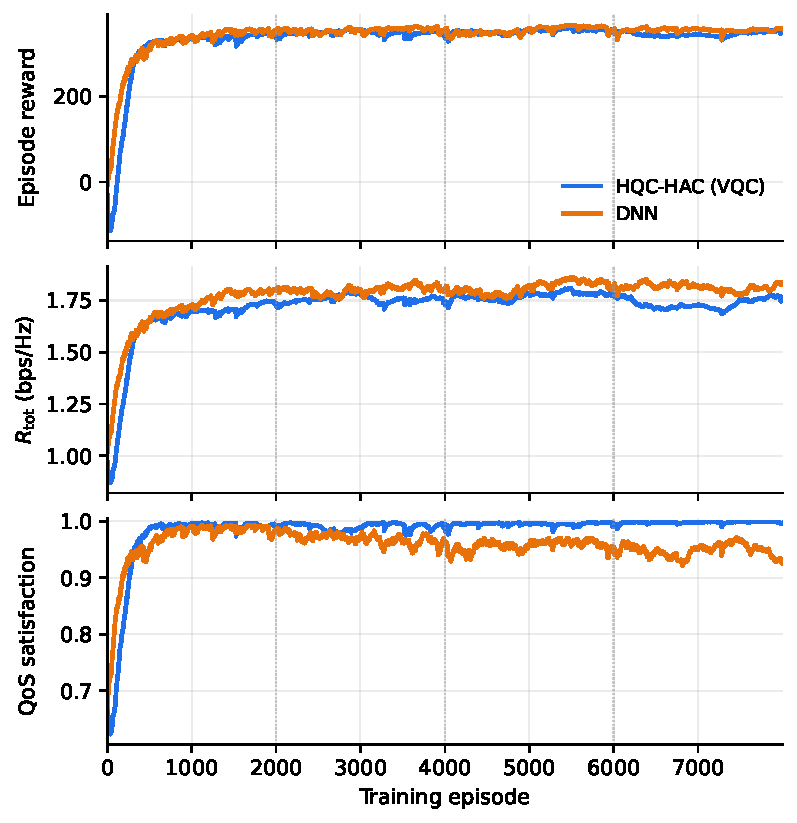
\includegraphics[width=0.45\textwidth]{figures/reward_log_case1}
\hfill
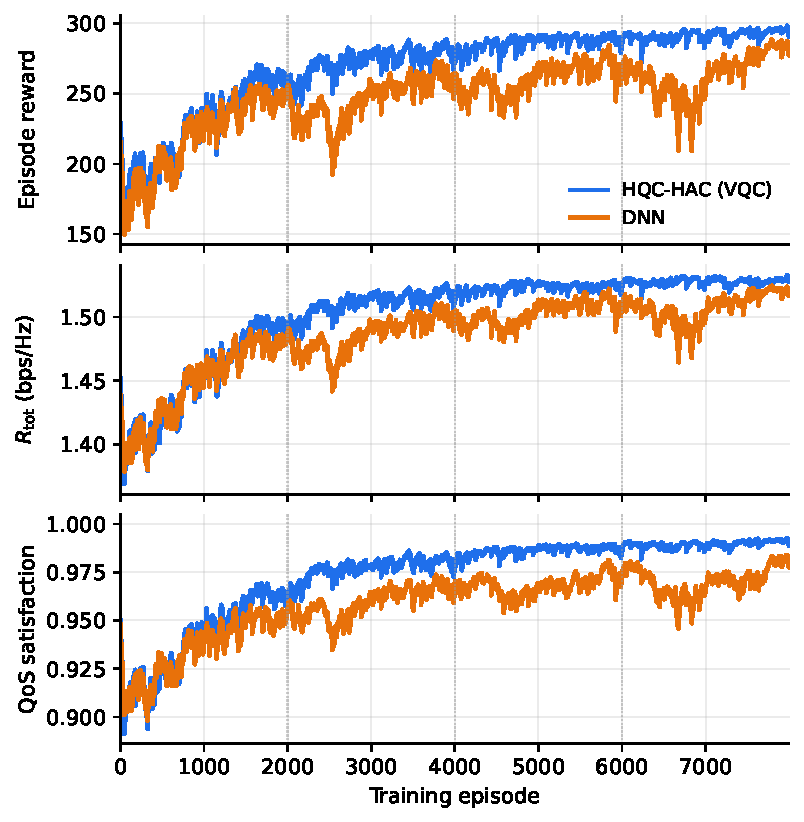
\includegraphics[width=0.45\textwidth]{figures/reward_log_case2}
\caption{Training curves for both problem sizes, showing mean episode return
over five training seeds under stochastic actions, with shaded regions
indicating one standard deviation.
Resumed training runs are stitched across segments; for $(K,M)=(5,1)$,
the VQC seed budget decreases after $10{,}000$ episodes as completed seeds
are excluded from the mean, while PPO-flat at $(10,2)$ averages two runs.
The curves are not directly comparable with Table~\ref{tab:case_main}, which reports greedy
inference at checkpoints selected under a $90\%$ QoS floor.}
\label{fig:reward_curves}
\end{figure*}


\begin{table}[t]
\centering
\caption{Performance under greedy inference at $P_S=50$\,dBm. All policies are evaluated
on the same $600$ test states ($3$ environment seeds $\times$ $200$ steps). Checkpoints
are selected on disjoint validation environments by maximizing greedy episode reward
subject to a $90\%$ QoS requirement. Learned rows are mean $\pm$ standard deviation over
five independent training seeds, the solvers being deterministic.}
\label{tab:case_main}
\footnotesize
\setlength{\tabcolsep}{3pt}
\resizebox{\linewidth}{!}{%
\begin{tabular}{lcccc}
\toprule
Policy & Reward & $R_{\mathrm{tot}}$ & QoS & Shortfall \\
\midrule
\multicolumn{5}{l}{\textit{Case 1} \, ($K{=}5$, $M{=}1$)} \\
HQC-HAC (VQC) & $490.3 \pm 22.1$ & $2.482 \pm 0.100$ & $92.4 \pm 3.2\%$ & $1.29\%$/$6.5{\cdot}10^{-4}$ \\
DNN         & $494.8 \pm 24.3$ & $2.501 \pm 0.121$ & $94.6 \pm 2.7\%$ & $1.00\%$/$5.0{\cdot}10^{-4}$ \\
PPO-flat    & $481.2 \pm 6.4$ & $2.417 \pm 0.035$ & $96.0 \pm 3.8\%$ & $0.23\%$/$1.1{\cdot}10^{-4}$ \\
AO          & $375.1$ & $1.876$ & $100.0\%$ & $0.00\%$/$0$ \\
Greedy      & $309.1$ & $1.549$ & $99.8\%$ & $0.06\%$/$0.3{\cdot}10^{-4}$ \\
Random      & $-307.6$ & $0.579$ & $47.8\%$ & $33.81\%$/$169{\cdot}10^{-4}$ \\
\midrule
\multicolumn{5}{l}{\textit{Case 2} \, ($K{=}10$, $M{=}2$)} \\
HQC-HAC (VQC) & $337.3 \pm 8.8$ & $1.742 \pm 0.021$ & $94.4 \pm 1.4\%$ & $0.88\%$/$4.4{\cdot}10^{-4}$ \\
DNN         & $337.5 \pm 2.3$ & $1.747 \pm 0.011$ & $92.1 \pm 2.0\%$ & $1.08\%$/$5.4{\cdot}10^{-4}$ \\
PPO-flat$^{\dagger}$ & $-367.1 \pm 53.7$ & $0.557 \pm 0.039$ & $47.2 \pm 3.1\%$ & $23.42\%$/$117{\cdot}10^{-4}$ \\
AO          & $330.1$ & $1.651$ & $100.0\%$ & $0.00\%$/$0$ \\
Greedy      & $281.2$ & $1.434$ & $99.4\%$ & $0.21\%$/$1.1{\cdot}10^{-4}$ \\
Random      & $-1582.9$ & $0.315$ & $19.6\%$ & $63.90\%$/$320{\cdot}10^{-4}$ \\
\bottomrule
\end{tabular}}

\vspace{2pt}
{\footnotesize $^{\dagger}$Two runs at learning rates $3{\cdot}10^{-4}$ and
$1{\cdot}10^{-4}$ rather than a five-seed mean.}
\end{table}



\subsection{Deployment Cost}
\label{sec:results_cost}

Table~\ref{tab:param_budget} decomposes both actors by role. The comparison is meaningful at
the level of the whole assignment actor, since the circuit
reaches its logits through a softmax layer that the classical policy network does not
require, so the $80$ and $96$ parameters of the quantum core are not by themselves a
substitute for the $1{,}410$ and $2{,}230$ of that network. Counted over the whole actor at
inference, where the encoder is included and the reconstruction decoder discarded, the
quantum pipeline is $9.2\times$ and $6.0\times$ smaller, and the complete policy is
$18.4\times$ and $33.2\times$ smaller than the flat baseline.

Table~\ref{tab:latency} reports what a decision and a training episode cost. At inference
the solver spends $23.93$ and $53.74$~ms per decision against between $0.42$ and $2.78$~ms
for the learned policies, but the more durable statement is the invocation count. AO calls
the rate kernel $482$ and $896$ times per action, growing with the user population, whereas
every learned policy calls it three times irrespective of scale. That count is independent
of language, machine, and, for the quantum actor, of the fact that its circuit is
simulated rather than executed.

The quantum actor requires $18.4$ and $25.2$~s per
episode against $1.7$ and $2.7$ for its classical counterpart and under $1.2$ for the flat
baseline,  and issues about $3.9{\cdot}10^{4}$ circuit
evaluations per episode. The solver requires no training whatsoever, so its entire cost falls at
inference. That asymmetry is precisely the trade an amortized policy makes, and it is
favourable only where the deployed system decides far more often than it is retrained.

\iffull
Two measurements delimit where the parameter advantage originates. Reducing the register
from eight qubits to six leaves performance inside the spread across training seeds, and
measuring only single-qubit $Z$ observables, eight of them in place of the $26$ of the
structured readout, does the same. The advantage therefore rests on how the state is
compressed for the circuit rather than on the circuit's expressive degrees of
freedom, which Section~\ref{sec:results_quantum} examines in detail.
\fi

\begin{table}[t]
\centering
\caption{Parameter budget across problem sizes $(K,M)$.
The upper block reports the \emph{assignment actor}, where the VQC and DNN
variants are directly substitutable; training parameters additionally include
the autoencoder decoder, which is discarded after training.
The lower block reports the complete inference policy, the level at which
PPO-flat is comparable because it jointly outputs all four decision variables.
}
\label{tab:param_budget}
\setlength{\tabcolsep}{4pt}
\begin{tabular}{@{}lcc@{}}
\toprule
 & $(5,1)$ & $(10,2)$ \\
\midrule
\multicolumn{3}{@{}l}{\emph{Assignment actor}} \\
\quad VQC core            & $80$   & $96$ \\
\quad Softmax policy layer & $391$  & $1{,}291$ \\
\quad AE encoder          & $272$  & $446$ \\
\quad AE decoder \emph{(training only)} & $561$ & $2{,}268$ \\
\cmidrule(l{1em}r){1-3}
\quad VQC, inference      & $743$      & $1{,}833$ \\
\quad VQC, training       & $1{,}304$  & $4{,}101$ \\
\quad DNN                 & $6{,}810$  & $11{,}086$ \\
\quad DNN\,/\,VQC (inference / training) & $9.2\times$/$5.2\times$ & $6.0\times$/$2.7\times$ \\
\midrule
\multicolumn{3}{@{}l}{\emph{Complete policy, inference}} \\
\quad HQC-HAC (VQC)       & $16{,}538$  & $21{,}831$ \\
\quad Classical (DNN)     & $23{,}629$  & $32{,}108$ \\
\quad PPO-flat            & $305{,}016$ & $725{,}239$ \\
\cmidrule(l{1em}r){1-3}
\quad PPO-flat\,/\,HQC-HAC & $18.4\times$ & $33.2\times$ \\
\bottomrule
\end{tabular}
\end{table}

\begin{table}[t]
\centering
\caption{Cost of one decision at inference and one training episode.
The upper half reports per-decision inference cost, while the lower half
reports per-episode training cost.
Within each half, the first block gives wall-clock time and the second
gives implementation-independent invocation counts.
Wall-clock values are medians.
AO is re-solved independently for each state and is not trained; hence,
training entries do not apply.}
\label{tab:latency}
% ── INFERENCE ──────────────────────────────────────────────────────────────
% Measured 2026-08-20 in ONE session, all eight cells together, machine idle
% (all 8 training processes SIGSTOPped), single thread
% (OPENBLAS/OMP/MKL_NUM_THREADS=1, CUDA_VISIBLE_DEVICES=''), same env seed,
% 300 timed decisions after 30 warm-up. Raw: analysis/data/latency_tabX_0820.txt
% Checkpoints: VQC r328/ep_02700 (C1), r291/ep_13700 (C2);
%              DNN r234/ep_07400 (C1), r231/ep_08700 (C2);
%              flat r301/ep_06000 (C1), r304 (C2).
% AO quoted at phase_sweeps=1, its measured J plateau (analysis/data/ao_sat_K*).
% ⚠ The previous version MIXED two sessions (latency_4method + latency_fill).
% ⚠ VQC timing is a CLASSICAL STATEVECTOR SIMULATION, not a hardware claim.
% ── TRAINING, wall-clock ───────────────────────────────────────────────────
% Median over archived CPU-backend runs, mean s/ep per run, runs with >500 ep:
%   C1 DNN  1.72 (IQR 1.53-2.56, n=12)   C1 VQC 18.38 (IQR 16.69-20.17, n=29)
%   C2 DNN  2.72 (IQR 2.44-3.03, n=12)   C2 VQC 25.23 (IQR 23.40-26.30, n=63)
%   flat from console-log cumulative elapsed:
%   C1 0.87 (0.81-1.06, n=11)            C2 1.19 (1.07-1.60, n=11)
% ⚠ GPU-backend runs are EXCLUDED: they sit at 60-98 s/ep because n_q=8 gives
%   only 2^8 amplitudes, so the GPU is pure kernel-launch overhead. Mixing them
%   in inflates the spread from 2.6x to 4.7x and is what made the archive look
%   unusable. Among CPU runs the IQR is +-6% of the median.
% Cross-check, live 549 s window 2026-08-20 with 3 of 8 cores busy:
%   VQC C1 (r418) 15.2, VQC C2 (r417) 22.9, flat C1 (r422) 0.67 -- all slightly
%   below the archive medians, consistent with less contention.
% ── TRAINING, circuit evaluations ──────────────────────────────────────────
% Per PPO minibatch the batched SPSA Jacobian costs 2*R*B circuit evaluations
% (RL/quantum_actor.py: spsa_jacobian_all_batch, 512 circuits at n_reps=4, B=64).
% With R=16, B=64, T=200, E=12, N_ep=6:
%   minibatches per update cycle = 12*200/64 * 6 = 225
%   SPSA evals per episode       = 225 * 2*16*64 / 12 = 38,400
%   rollout forward evals        = 200
%   total                        ~ 3.9e4 per episode, IDENTICAL at both cases
%   (it depends only on T, E, B, N_ep, R -- the wall-clock gap between cases is
%   classical-side work, not circuit work).
% Parameter-shift would cost 2*n_eta*B with n_eta = 2(L+1)n_q, i.e. 3.0x (C1)
% and 4.0x (C2) more, matching the ratio quoted in Section IV-E.
\setlength{\tabcolsep}{4pt}
\small
\begin{tabular}{llcccc}
\toprule
 & & AO & PPO-flat & DNN & VQC \\
\midrule
\multicolumn{6}{@{}l}{\emph{Inference, per decision}} \\
\multirow{2}{*}{Latency (ms)}
  & $(5,1)$  & $23.93$ & $\mathbf{0.42}$ & $0.60$ & $1.94$ \\
  & $(10,2)$ & $53.74$ & $\mathbf{0.66}$ & $0.85$ & $2.78$ \\
\cmidrule(l{1em}r){1-6}
\multirow{2}{*}{Rate-kernel evals}
  & $(5,1)$  & $482$ & $\mathbf{3}$ & $\mathbf{3}$ & $\mathbf{3}$ \\
  & $(10,2)$ & $896$ & $\mathbf{3}$ & $\mathbf{3}$ & $\mathbf{3}$ \\
\midrule
\multicolumn{6}{@{}l}{\emph{Training, per episode}} \\
\multirow{2}{*}{Wall-clock (s)}
  & $(5,1)$  & n/a & $\mathbf{0.87}$ & $1.72$ & $18.38$ \\
  & $(10,2)$ & n/a & $\mathbf{1.19}$ & $2.72$ & $25.23$ \\
\cmidrule(l{1em}r){1-6}
\multirow{2}{*}{Circuit evals}
  & $(5,1)$  & n/a & n/a & n/a & $3.9{\cdot}10^{4}$ \\
  & $(10,2)$ & n/a & n/a & n/a & $3.9{\cdot}10^{4}$ \\
\bottomrule
\end{tabular}
\end{table}


\begin{table*}[!t]
\centering
\caption{Zero-shot generalization under distribution shifts for both cases.
Policies are trained at the base operating point
($P_S=50$\,dBm, $\kappa=0.05$, $\sigma^2=10$\,dBW, user speed $1.5$\,m/s)
and evaluated without retraining under shifted environments, while AO is
re-optimized for each shifted state.
Combined-A denotes $\{P_S=40$\,dBm, $\kappa=0.10$, speed $=3$\,m/s$\}$ and
Combined-B denotes $\{P_S=60$\,dBm, $\kappa=0.20$, speed $=6$\,m/s,
$\sigma^2=16$\,dBW$\}$.
Operating points with $P_S\neq50$\,dBm are retrained and reported separately,
as transmit power is a deployment parameter rather than a runtime
environmental variable.
The $N$-shift rows are zero-shot for the hierarchical actors, whose
affinity map and phase sub-actor do not depend explicitly on $N$; PPO-flat
is retrained because its unaggregated channel input dimension changes with
$N$.
The $90\%$ QoS floor is applied only to base-row checkpoint selection;
shifted rows use unconstrained argmax return.
A dagger indicates QoS below $90\%$, for which the corresponding rate is not directly comparable with entries satisfying the QoS floor.}
\label{tab:abl_genshift}
\setlength{\tabcolsep}{3pt}
\scriptsize
\begin{tabular}{lcccccccccccc}
\toprule
 & \multicolumn{3}{c}{AO} & \multicolumn{3}{c}{PPO-flat} & \multicolumn{3}{c}{DNN} & \multicolumn{3}{c}{HQC-HAC (VQC)} \\
\cmidrule(lr){2-4}\cmidrule(lr){5-7}\cmidrule(lr){8-10}\cmidrule(lr){11-13}
Shift & $R_{\mathrm{tot}}$ & QoS & Reward & $R_{\mathrm{tot}}$ & QoS & Reward & $R_{\mathrm{tot}}$ & QoS & Reward & $R_{\mathrm{tot}}$ & QoS & Reward \\
\midrule
\multicolumn{13}{l}{\emph{Case~1 ($K=5$, $M=1$)}} \\
Base & $1.8366$ & $100.0$\% & $367.3$ & $2.4658$ & $93.6$\% & $489.3$ & $2.4829$ & $94.4$\% & $\mathbf{491.1}$ & $2.4653$ & $92.3$\% & $486.5$ \\
\cmidrule(lr){1-13}
$P_S=40$ & $1.3278$ & $100.0$\% & $265.3$ & $1.0812$ & $92.7$\% & $197.0$ & $1.8350$ & $76.9$\%$^{\dagger}$ & $\mathbf{329.1}$ & $1.7917$ & $78.8$\%$^{\dagger}$ & $321.5$ \\
$P_S=60$ & $1.9928$ & $100.0$\% & $398.6$ & $2.9638$ & $97.5$\% & $\mathbf{587.3}$ & $2.8024$ & $94.3$\% & $556.5$ & $2.7942$ & $95.3$\% & $556.3$ \\
$P_S=70$ & $2.0809$ & $100.0$\% & $416.2$ & $10.2956$ & $99.9$\% & $\mathbf{2059.0}$ & $3.8151$ & $81.7$\%$^{\dagger}$ & $596.2$ & $3.9302$ & $80.5$\%$^{\dagger}$ & $601.8$ \\
\cmidrule(lr){1-13}
$N=16$ & $1.8216$ & $100.0$\% & $364.3$ & $2.1698$ & $92.5$\% & $430.0$ & $2.3710$ & $93.2$\% & $\mathbf{466.3}$ & $2.3449$ & $92.1$\% & $461.9$ \\
$N=32$ & $1.9105$ & $100.0$\% & $382.1$ & $2.6684$ & $90.4$\% & $\mathbf{531.5}$ & $2.5764$ & $96.0$\% & $512.2$ & $2.5720$ & $92.9$\% & $508.8$ \\
\cmidrule(lr){1-13}
$\kappa=0.10$ & $1.8369$ & $100.0$\% & $367.4$ & $2.4667$ & $93.6$\% & $489.5$ & $2.4808$ & $94.3$\% & $\mathbf{490.2}$ & $2.4661$ & $92.3$\% & $486.7$ \\
$\kappa=0.15$ & $1.8365$ & $100.0$\% & $367.3$ & $2.4662$ & $93.5$\% & $\mathbf{489.4}$ & $2.4722$ & $94.1$\% & $487.1$ & $2.4665$ & $92.2$\% & $486.5$ \\
$\kappa=0.20$ & $1.8366$ & $100.0$\% & $367.3$ & $2.4659$ & $93.5$\% & $\mathbf{489.2}$ & $2.4588$ & $93.0$\% & $478.7$ & $2.4654$ & $92.2$\% & $486.3$ \\
\cmidrule(lr){1-13}
$\sigma^2=13$ & $1.8232$ & $100.0$\% & $364.6$ & $2.4425$ & $92.9$\% & $484.1$ & $2.4664$ & $94.0$\% & $\mathbf{487.4}$ & $2.4507$ & $92.0$\% & $483.0$ \\
$\sigma^2=16$ & $1.8104$ & $100.0$\% & $362.1$ & $2.4203$ & $92.1$\% & $478.8$ & $2.4506$ & $93.7$\% & $\mathbf{483.6}$ & $2.4337$ & $91.7$\% & $479.0$ \\
\cmidrule(lr){1-13}
Combined-A & $1.1427$ & $98.9$\% & $225.2$ & $1.0048$ & $91.2$\% & $173.2$ & $1.7265$ & $78.0$\%$^{\dagger}$ & $\mathbf{308.8}$ & $1.7431$ & $76.7$\%$^{\dagger}$ & $307.0$ \\
Combined-B & $1.7818$ & $100.0$\% & $356.3$ & $2.5592$ & $97.4$\% & $504.7$ & $2.8937$ & $95.4$\% & $\mathbf{574.6}$ & $2.8356$ & $95.4$\% & $564.5$ \\
\cmidrule(lr){1-13}
\multicolumn{13}{l}{\emph{Case~2 ($K=10$, $M=2$)}} \\
Base & $1.6515$ & $100.0$\% & $330.3$ & $0.5874$ & $54.4$\%$^{\dagger}$ & $-326.5$ & $1.7522$ & $91.5$\% & $\mathbf{337.4}$ & $1.7397$ & $94.4$\% & $337.1$ \\
\cmidrule(lr){1-13}
$P_S=40$ & $1.2979$ & $93.8$\% & $\mathbf{240.1}$ & $0.8579$ & $76.3$\%$^{\dagger}$ & $-244.1$ & $0.9825$ & $92.7$\% & $162.0$ & $0.9786$ & $93.2$\% & $162.3$ \\
$P_S=60$ & $1.7418$ & $100.0$\% & $348.4$ & $2.6097$ & $89.7$\%$^{\dagger}$ & $\mathbf{503.8}$ & $2.2359$ & $87.4$\%$^{\dagger}$ & $438.7$ & $2.1907$ & $92.0$\% & $432.9$ \\
$P_S=70$ & $1.7581$ & $100.0$\% & $351.6$ & $10.1880$ & $98.0$\% & $\mathbf{2036.7}$ & $2.2988$ & $87.7$\%$^{\dagger}$ & $454.3$ & $2.2860$ & $91.1$\% & $453.3$ \\
\cmidrule(lr){1-13}
$N=16$ & $1.6341$ & $100.0$\% & $\mathbf{326.8}$ & $0.5771$ & $51.5$\%$^{\dagger}$ & $-283.0$ & $1.6688$ & $89.8$\%$^{\dagger}$ & $309.5$ & $1.6594$ & $92.6$\% & $308.6$ \\
$N=32$ & $1.6575$ & $100.0$\% & $331.5$ & $0.5138$ & $43.5$\%$^{\dagger}$ & $-397.4$ & $1.7754$ & $93.1$\% & $\mathbf{345.4}$ & $1.7568$ & $95.3$\% & $345.1$ \\
\cmidrule(lr){1-13}
$\kappa=0.10$ & $1.6513$ & $100.0$\% & $330.3$ & $0.5874$ & $54.4$\%$^{\dagger}$ & $-326.4$ & $1.7516$ & $91.5$\% & $\mathbf{337.4}$ & $1.7380$ & $94.3$\% & $336.3$ \\
$\kappa=0.15$ & $1.6513$ & $100.0$\% & $330.3$ & $0.5873$ & $54.4$\%$^{\dagger}$ & $-326.5$ & $1.7495$ & $91.5$\% & $\mathbf{336.2}$ & $1.7321$ & $94.2$\% & $334.5$ \\
$\kappa=0.20$ & $1.6508$ & $100.0$\% & $330.2$ & $0.5872$ & $54.4$\%$^{\dagger}$ & $-326.4$ & $1.7478$ & $91.4$\% & $\mathbf{335.5}$ & $1.7239$ & $94.0$\% & $331.9$ \\
\cmidrule(lr){1-13}
$\sigma^2=13$ & $1.6410$ & $100.0$\% & $328.2$ & $0.5909$ & $55.3$\%$^{\dagger}$ & $-337.4$ & $1.7321$ & $91.2$\% & $\mathbf{332.3}$ & $1.7157$ & $94.2$\% & $331.4$ \\
$\sigma^2=16$ & $1.6309$ & $100.0$\% & $326.2$ & $0.5943$ & $56.0$\%$^{\dagger}$ & $-347.2$ & $1.7134$ & $90.8$\% & $\mathbf{327.3}$ & $1.6942$ & $93.9$\% & $326.3$ \\
\cmidrule(lr){1-13}
Combined-A & $1.0949$ & $93.6$\% & $\mathbf{201.5}$ & $0.8163$ & $72.8$\%$^{\dagger}$ & $-317.3$ & $0.9646$ & $91.7$\% & $159.2$ & $0.9632$ & $92.3$\% & $158.4$ \\
Combined-B & $1.6233$ & $100.0$\% & $324.4$ & $2.7734$ & $84.2$\%$^{\dagger}$ & $\mathbf{503.3}$ & $2.3042$ & $89.8$\%$^{\dagger}$ & $453.0$ & $2.2558$ & $93.5$\% & $445.1$ \\
\bottomrule
\end{tabular}
\end{table*}

\subsection{Robustness to Distribution Shift}
\label{sec:results_shift}

Table~\ref{tab:abl_genshift} evaluates every policy under thirteen shifts applied after
training. Quadrupling the CSI error from
$\kappa=0.05$ to $0.20$ costs the quantum actor $0.04\%$ of its sum-rate at $(5,1)$ and
$0.7\%$ at $(10,2)$, and raising the noise variance from $10$ to $16$~dB$^2$ costs $1.1\%$
and $2.3\%$. Both learned actors therefore degrade gracefully under exactly the
perturbations that imperfect CSI is meant to model.

Transmit power is a different axis, a deployment parameter rather than a runtime one, so
those rows are retrained at their own budget. Both learned actors retain an advantage down
to $50$~dBm, while at $40$~dBm and under combined-A the solver leads on both metrics at
once.

PPO-flat fails discontinuously. At $(10,2)$ it falls below the solver at ten of thirteen
shifts, and its column is static across the base point and all five CSI and noise shifts,
 so the failure is one break at the base operating
point rather than a response to the shifts. The same table nevertheless places it ahead of
every other method once the budget is generous, at $503.8$ and $2036.7$ against $438.7$ and
$454.3$ for the classical actor at $60$ and $70$~dBm. The hierarchical actors fall below the
solver only where the solver itself leaves $100\%$ QoS. Daggers $^{\dagger}$ mark operating points 
below the $90\%$ floor, twenty-two of the seventy-eight
learned entries. At $(10,2)$ the quantum actor clears it at all thirteen shifts and
PPO-flat at one.


\iffull

\subsection{What the Quantum Resources Contribute}
\label{sec:results_quantum}

Table~\ref{tab:abl_modelscale} varies the decision core along three axes while holding the
encoder and the policy layer fixed, so the parameter column counts the substitutable module
alone on both sides. Reducing the register from eight qubits to six moves $R_{\mathrm{tot}}$
from $1.742 \pm 0.021$ to $1.735$, inside the spread across training seeds, at a core of
$72$ parameters instead of $96$. Removing the entangling bridges while holding the
parameter count and the readout unchanged yields $1.703$, again within the seed spread,
although that run used a shorter training budget than the reference chain and the
comparison should be read accordingly.

Table~\ref{tab:abl_readout} varies the measured observable set at a fixed register. The
sets are not nested and their sizes do not rank them, so each case is reported separately.
At $(10,2)$, measuring eight single-qubit $Z$ observables reaches $1.749$ at $95.9\%$ QoS
against $1.742 \pm 0.021$ at $94.4 \pm 1.4\%$ for the structured readout with $26$.

Taken together these measurements locate the contribution. The autoencoder is indispensable,
since a direct encoding would demand $17$ and $44$ qubits at the two scales and place
state-vector simulation with per-step gradients out of reach. The register size, the
observable set and the two-qubit correlations are, within the resolution of these
experiments, inert.

\begin{table}[t]
\centering
\caption{Ablation of the \emph{decision core} at Case~2. All rows share the same
autoencoder encoder and softmax policy layer, so the parameter column counts the
substitutable decision module alone on both sides. The two reference rows are the
Case-2 main-table entries; each block below varies one axis away from the quantum
reference and omits the reference setting itself. Rows carrying a spread are
five-training-seed means, the rest are single seeds.}
\label{tab:abl_modelscale}
% Filled 2026-08-20/21:
%   Reference VQC  = Table VII HQC-HAC row (5 seeds), n_q=8 L=3 with CZ bridges
%   Reference MLP  = Table VII DNN row (5 seeds), pol_hidden=[40]; core 2,230 from
%                    analysis/probe_param_count.py (enc[128] pol[40], total 11,086)
%   n_q=6          = r396/ep_19200, 1 seed. QoS>=90 over 26 ckpts on val 7/21/99
%                    (pick_r396_nq6.txt), scored on test 42/43/44.
%   no CZ bridges  = r322/ep_01700, 1 seed. --no-entangle; probe_param_count
%                    confirms an IDENTICAL budget (core 96, total 1,833), so this
%                    is a pure structural ablation at constant capacity.
%                    All 27 ckpts cleared the floor; best 329.93 on validation.
% ⚠ r322 ran only 2700 episodes against the reference chain's 10300-19800, so part
%   of its 1.742 -> 1.703 shortfall (about 1.7 sigma) is budget, not entanglement.
%   Re-run at the full budget before making this a headline number.
% ⚠ r306 also carries no_entangle=True but its log header still prints the CZ
%   bridges; it predates the summary fix at train.py:1954 and cannot be trusted.
% ⚠ n_q=10 has NO usable run: r392/393/395 died mid-flight, r148/277/295 predate
%   the per-element refactor, r416 is at 5.8%% with a 30-day ETA at 148 s/ep.
% ⚠ The L rows are pending r426 (L=1) and r427 (L=2); L=4 and L=6 unstarted.
% ⚠ The other MLP widths (r138 64x64, r139/140 64x32, r141 32x16, r142 16x8) are
%   ALL pre-refactor and need retraining under --pol-hidden.
\setlength{\tabcolsep}{5pt}
\begin{tabular}{llccc}
\toprule
Decision core & Configuration & Params & $R_{\mathrm{tot}}$ & QoS \\
\midrule
\multicolumn{5}{@{}l}{\emph{Reference}} \\
\quad VQC           & $n_q{=}8$, $L{=}3$, entangled & $96$      & $1.742 \pm 0.021$ & $94.4 \pm 1.4\%$ \\
\quad Classical MLP & $(40)$                        & $2{,}230$ & $1.747 \pm 0.011$ & $92.1 \pm 2.0\%$ \\
\midrule
\multicolumn{5}{@{}l}{\emph{Classical width}} \\
\quad & $(256,128)$ & \emph{---} & \emph{---} & \emph{---} \\
\quad & $(128,128)$ & \emph{---} & \emph{---} & \emph{---} \\
\quad & $(64,64)$   & \emph{---} & \emph{---} & \emph{---} \\
\quad & $(64,32)$   & \emph{---} & \emph{---} & \emph{---} \\
\quad & $(32,16)$   & \emph{---} & \emph{---} & \emph{---} \\
\midrule
\multicolumn{5}{@{}l}{\emph{Circuit depth} ($n_q{=}8$)} \\
\quad & $L=1$ & $64$  & \emph{---} & \emph{---} \\
\quad & $L=2$ & $80$  & \emph{---} & \emph{---} \\
\quad & $L=4$ & $112$ & \emph{---} & \emph{---} \\
\quad & $L=6$ & $144$ & \emph{---} & \emph{---} \\
\midrule
\multicolumn{5}{@{}l}{\emph{Register size} ($L{=}3$)} \\
\quad & $n_q=6$  & $72$  & $1.735$    & $94.6\%$ \\
\quad & $n_q=10$ & $120$ & \emph{---} & \emph{---} \\
\midrule
\multicolumn{5}{@{}l}{\emph{Entanglement} ($n_q{=}8$, $L{=}3$)} \\
\quad & no CZ bridges & $96$ & $1.703$ & $94.6\%$ \\
\bottomrule
\end{tabular}
\end{table}


\subsection{Representation Quality}
\label{sec:results_repr}

Table~\ref{tab:abl_repr} asks how much assignment-relevant information each latent carries,
independently of the policy that consumes it. A lightweight classical probe is trained to
recover the oracle assignment from frozen representations on a common held-out state set,
so the comparison isolates the encoding from the downstream actor. The quantum and
classical encoders reach comparable accuracy, and both are close to what the raw state and
the full channel afford. The encoders therefore concentrate rather than merely preserve the
information the assignment depends on, and the residual gap between a probe and the live
policy is one of credit assignment during training rather than of representational
capacity.

\begin{table}[t]
\centering
\caption{Representation quality (Case~2): supervised recovery of the oracle assignment from frozen
representations on a common held-out state set ($N=384$). Both actors encode the identical
states, and the resulting latent representations are evaluated independently of the downstream
policy. Exact accuracy measures full assignment recovery, while IRS/direct accuracy measures
correct classification into IRS-assisted versus direct transmission.
}
% !! STALE NUMBERS — measured BEFORE the per-element g_RU refactor, the R_k^{\min}=0.05
% !! recalibration and the power-head fix, and with n_q=12 rather than the n_q=8
% !! used everywhere else in this paper. They are NOT the current configuration.
% !! Re-measure once the VQC multi-seed runs finish; every row here needs a
% !! final VQC checkpoint, which is why they could not be updated with the
% !! parameter budget above.
\label{tab:abl_repr}
\begin{tabular}{lcc}
\toprule
Representation & Exact acc. & IRS/direct acc. \\
\midrule
$\mathbf{z}_t$ (VQC-AE)             & $96.2\%$ & $97.1\%$ \\
$\mathbf{z}_t$ (DNN)                & $95.8\%$ & $96.8\%$ \\
Raw state $\mathbf{s}_t$            & $95.8\%$ & $97.0\%$ \\
Full channel                        & $95.9\%$ & $97.1\%$ \\
\bottomrule
\end{tabular}
\end{table}
\fi

\subsection{Budget Allocation Policy}
\label{sec:results_alloc}

The comparisons so far report what each policy achieves; Fig.~\ref{fig:power_ladder}
reports how, as the Lorenz curve of the private power across users at four transmit
budgets. The solver lies on the diagonal at every rung, Gini $0.00$ throughout, because it
divides private power equally by construction. Whatever the learned policies gain on the
power axis of Section~\ref{sec:pareto_frontier} is gained here.

For the hierarchical actors the dependence on the budget is not monotone. Concentration
attains a minimum at intermediate budgets, $0.10$ and $0.07$ at $(5,1)$ and $60$~dBm, and
rises at both extremes, to $0.50$ for either actor at $40$~dBm and to $0.14$ and $0.19$ at
$70$~dBm. At the low end no even split brings any user
to its demand, so serving a subset well is what the reward prefers; at the high end the
shortfall penalty is capped at $\lambda_D$ per withheld user while the rate term grows with
$P_S$, so withholding eventually pays for itself. This is the trade-off of
Section~\ref{sec:pareto_frontier} seen along the power budget rather than along $\lambda_D$.

PPO-flat shows only the second rise, and without bound. At $40$~dBm it is the least
concentrated of the three learned policies at both scales; at $70$~dBm it places the entire
private budget on one user. It answers the incentive that rewards concentration where the
budget is large enough that the demand is met whatever the allocation, and not the one that
punishes it where the budget is tight. That single mechanism accounts for both of its
anomalies, the collapse at $(10,2)$ in Table~\ref{tab:case_main} and the lead at $60$ and
$70$~dBm in Table~\ref{tab:abl_genshift}, each being the same policy answered by a
different budget.

\begin{figure*}[t]
\centering
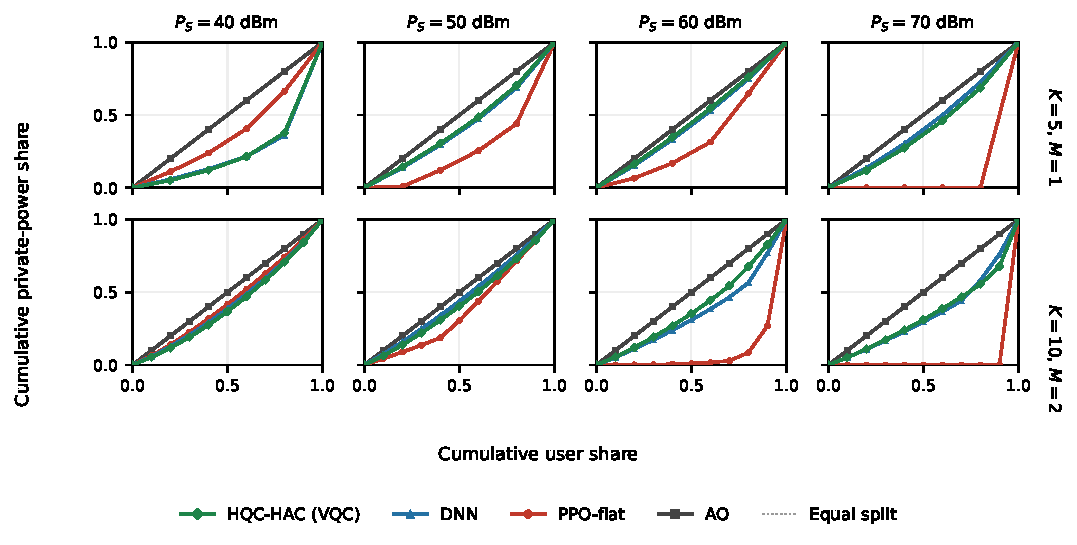
\includegraphics[width=\textwidth]{figures/power_ladder}
\caption{Lorenz curves of private-power allocation across transmit-power
budgets. Users are ordered by received private power; the diagonal denotes
equal allocation, and the area between a curve and the diagonal gives the
Gini coefficient. The common stream is omitted because it is allocated per
group rather than per user. Curves use the greedy checkpoints of Table~VI.}
\label{fig:power_ladder}
\end{figure*}

\section{Rate--QoS Frontier}
\label{sec:pareto_frontier}

The policies of Section~\ref{sec:results_main} settle at different service levels, so the
reference they are measured against has to be defined at a service level too. For a fixed
environment let
\begin{equation}
F(q) \;=\; \max_{\boldsymbol{\varphi},\,\boldsymbol{\Phi},\,\mathbf{w},\,\mathbf{C}}\
\mathbb{E}\bigl[R_{\mathrm{tot}}\bigr]
\quad \text{s.t.} \quad \mathbb{E}[\mathrm{QoS}] \ge q ,
\label{eq:frontier}
\end{equation}
the largest mean sum-rate attainable at mean QoS $q$ under the constraints of (P0). The
constraint binds the mean, as Table~\ref{tab:case_main} reports it. Constraining every state
separately defines a different and strictly lower quantity, since it forbids trading service
between states, and evaluating one against the other is a common way to overstate how close a
policy sits. We obtain $F$ on the $600$ test states of Table~\ref{tab:case_main} by
enumerating every assignment, solving the phase exactly for each, sweeping the power split on
a grid, filling $C_k$ by demand, and tracing the upper envelope by Lagrangian sweep, with
decisions taken on $\hat{g}$ and scored on $g$ as in training. Because the power search is a
grid rather than a full optimization, $F$ is an achievable lower bound on the true frontier.

\iffull
In the high-power regime the SINRs reduce to $x_k/(1-x_k-y_{g(k)})$ and $y_g/(1-y_g)$ in the
power fractions $x_k=w_{p,k}/P_S$ and $y_g=w_c^g/P_S$: the channel magnitudes cancel and the
frontier is set by how many users are served and how the unit budget is divided. Under an
equal split across $m$ served users the private sum-rate is the concentration identity
$R(m)=m\log_2\frac{m}{m-1}$, decreasing in $m$ with floor $1/\ln 2$.
\fi

\begin{figure*}[t]
\centering
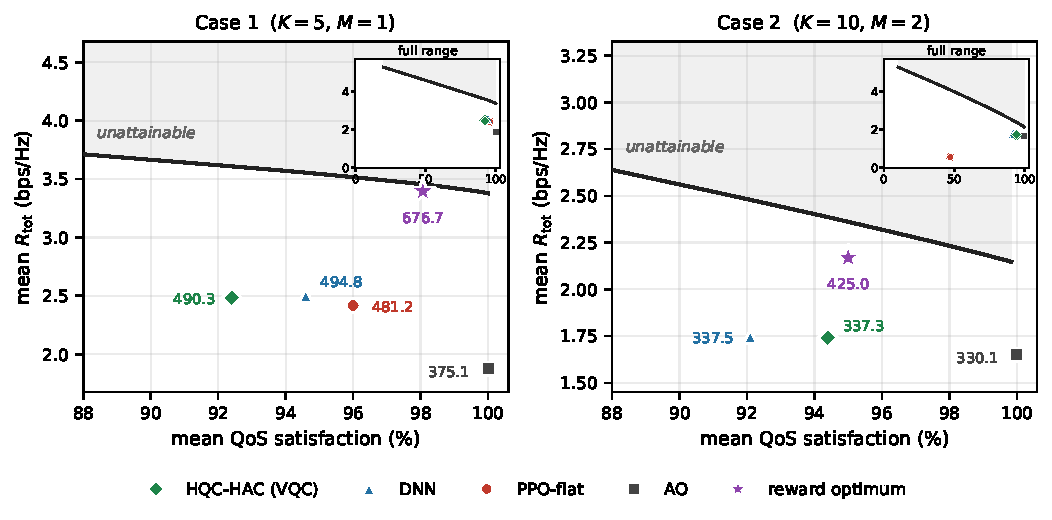
\includegraphics[width=\textwidth]{figures/pareto_frontier}
\caption{Rate--QoS frontier and policy operating points for 600 test states
per case. The frontier in~\eqref{eq:frontier} is obtained by a Lagrangian sweep over the
achievable sets; since assignment is exhaustively enumerated and phase is
solved exactly, while power splitting is grid-swept, it provides an
achievable lower bound, with the shaded region unattainable under this
construction. Markers denote the greedy-inference operating points from
Table~\ref{tab:case_main}, annotated by episode return, while stars indicate the
reward-optimal operating points over the same achievable sets.
The inset shows the full QoS range for Case~2, including PPO-flat.}
\label{fig:pareto}
\end{figure*}

Fig.~\ref{fig:pareto} shows the frontier is shallow across the high-service
region and steepens only once QoS is allowed to fall, the signature of an
interference-limited link, in which concentrating power raises one user's rate and everyone
else's interference with it. Serving every user is not merely costly but sometimes
infeasible, attainable in $99.5\%$ of states at $(5,1)$ and in $87.3\%$ at $(10,2)$. Of the
$3.38$ and $2.15$~bps/Hz the frontier reaches at full service, the equal-split identity
accounts for $1.61$ and $1.52$; the remainder is bought by dividing power unequally, the axis
on which a solver that splits private power evenly by construction cannot compete.

All four policies lie well below the frontier, and their distances from it are not read the
same way. The solver is pinned to the right-hand edge, because its common-rate allocation is
ordered by service and it therefore ends at full QoS whatever the channel, and that edge is
where the frontier is lowest. Proximity to $F$ is accordingly not the figure of merit, since
$F$ maximizes rate at a fixed service level whereas every policy here maximizes the
QoS-penalized reward of~\eqref{eq:reward}. The two targets are distinct, and the point the
reward itself selects lies at $98.1\%$ and $95.0\%$ QoS rather than at $100\%$. Measured on
that objective the learned actors reach $73.1\%$ and $79.4\%$ of the attainable return,
against $55.4\%$ and $77.7\%$ for the solver.

The operating point is therefore chosen by $\lambda_D$ rather than arrived at by accident.
Withholding service from one user costs $\lambda_D\hat{p}$ with
$\hat{p}=\bigl(R_k^{\min}/(R_k^{\min}+\epsilon_{\mathrm q})\bigr)^2$, so the serve-all optimum
takes over above
\begin{equation}
\lambda_{\mathrm{crit}}
= \frac{V^*_{\mathrm{rate}} - R^*(K)}{(K-1)\,\hat{p}},
\qquad
V^*_{\mathrm{rate}} = \mathbb{E}\bigl[\log_2(1+\Gamma_{\max})\bigr],
\label{eq:lcrit}
\end{equation}
$V^*_{\mathrm{rate}}$ being the rate of placing the whole budget on the strongest link, the
one configuration free of intra-system interference. Measured,
$\lambda_{\mathrm{crit}}=1.74$ at $(5,1)$ and $1.01$ at $(10,2)$, which places the training
value $\lambda_D=1.5$ on opposite sides of the two cases. At the smaller scale the reward's
global optimum is the degenerate single-user concentration, and entropy regularization is
what holds the policy in the serve-all region; at the larger scale the reward already prefers
serving everyone.

\iffull
That the reward optimum sits below full service follows from the penalty rather than from any
shortage of power. Its marginal cost $2\lambda_D t/(R_k^{\min}+\epsilon_{\mathrm q})^2$
vanishes as the shortfall $t\to0$, so the reward-optimal common-rate split is a water-filling
solution, the shares solving $\sum_{k\in\mathcal{K}_g}(\varsigma_k-t^\star)^+ = R_{c,g}$ for a
common level $t^\star$, which settles the weakest users marginally below their demand. Full
service and reward optimality are therefore separate targets at every $\lambda_D$, and the
comparison in Fig.~\ref{fig:pareto} is made at matched service for that reason.
\fi

\section{Discussion}
\label{sec:discussion}

The evidence assembled here supports a claim of feasibility and efficiency rather than of
quantum advantage on the task itself. At both scales the variational actor and the classical
actor it replaces are separated by less than a quarter of the spread across training seeds,
which is what the prevailing prior for parametrized quantum policies
anticipates~\cite{jerbi2021parametrized,bowles2024better}. What distinguishes them is the budget at which
that performance is obtained. Set against a solver re-run at
every channel realization~\cite{tan2025flexible}, the learned policy converts a recurring
per-state cost into a single offline one.

The measurements also separate what the design owes to compression from what it owes to the
circuit. The autoencoder is indispensable because it decouples the register from the problem
size, a direct angle encoding of the affinity state requiring $17$ and $44$ qubits at the two
scales and $81$ at $K{=}15$ while the register stays at eight throughout. Within the
resolution of these experiments the parameter saving follows from that compression rather
than from the expressive degrees of freedom of the circuit itself. \iffull
Three measurements delimit that statement. Reducing the
register from eight qubits to six, and measuring eight single-qubit $Z$ observables in place
of the $26$ of the structured readout, each leave the sum-rate inside the seed
spread, as does removing the entangling bridges at a fixed parameter count
(Section~\ref{sec:results_quantum}). We report this as a negative result about the circuit
rather than about the framework. It locates the parameter saving in how the state is
compressed for the register rather than in the correlations the register is able to
represent, and it suggests that the assignment problem at these scales is not one whose
structure a shallow entangling ansatz exploits.
\fi

That saving carries a cost, and the regime in which it is repaid is narrow. Training the
quantum actor costs roughly an order of magnitude more per episode than training its
classical counterpart. The
margin over the solver is bounded in a second sense. It is widest where the power budget is
generous and reverses at $40$~dBm and under the combined shift, the two operating points at
which the solver itself ceases to reach full service, so the learned policies fall behind
where the problem becomes constrained rather than uniformly.

\section{Limitations}
\label{sec:limitations}

The quantum actor is evolved by state-vector simulation, so gate noise, the
sampling error remaining beyond the shot budget modelled here, and compilation
onto a device topology all lie outside the measurement, and the inference figures
are algorithmic rather than hardware results. An eight-qubit register is within
reach of present devices, but the ${\approx}3.9{\cdot}10^{4}$ circuit evaluations
each training episode consumes would be device time rather than simulated time,
and it is that budget, not the register width, that separates the framework from
execution on physical hardware.

The parameter ratio depends on where the boundary between the quantum and
classical parts is drawn, falling to roughly $1.4\times$ once the classical
sub-actors the two arms share are counted. Every learned row averages
five training seeds, at which resolution the QoS separation at $(10,2)$ is the
sole difference between the two instantiations exceeding two standard errors.

The system model is restricted in two further respects. A single-antenna
satellite admits only scalar precoding, so the spatial degrees of freedom of a
multibeam payload, and the inter-group interference management they would afford,
lie outside the formulation. The policy is also trained for a fixed user
population and panel count, and the study spans two network scales and one
channel family, so the narrowing of the margin over the solver with scale is
observed rather than established.

\section{Conclusion}
\label{sec:conclusion}

We presented HQC-HAC, a hybrid quantum--classical hierarchical actor--critic for sum-rate
maximization in IRS-assisted grouped-RSMA integrated satellite--terrestrial networks. The
formulation casts the joint assignment, phase, power, and common-rate problem as a sequential
dependency chain under QoS, discrete-phase, blockage, and imperfect-CSI constraints. A
variational quantum circuit resolves the combinatorial $(M{+}1)^K$ assignment, three
classical sub-actors resolve the factorable low-level controls, and an autoencoder compresses
the state so that the register size follows the design rather than the network size. Across
two scales the method matches a classical actor of identical role, input, and output to
within the spread across training seeds while using $9.2\times$ and $6.0\times$ fewer
parameters in the actor the two share, and it answers each channel realization with three
evaluations of the rate kernel rather than the several hundred a per-state solver requires.
It exceeds that solver by $31\%$ at the smaller scale, the margin narrowing to within one
standard deviation at the larger one.
\fullonly{The ablations attribute the outcome to the compression rather than to the
register size, the observable set, or the entangling structure, none of which alters
performance measurably at these scales. }Future work includes execution on quantum hardware, a multibeam payload, a
user population that varies without retraining, and a systematic sweep of circuit depth
against classical width at matched budgets.

\bibliographystyle{IEEEtran}
\bibliography{reference}

\iffull
\appendices
\section{Architectural and Autoencoder Ablations}
\label{sec:ablation}

% ---- A2 : autoencoder latent compression -- maps to C3 --------------------
\subsection{Autoencoder Latent Compression}
\label{sec:abl_ae} 
The AE compresses the high-dimensional state into a latent $\mathbf{z}_t\in\mathbb{R}^{2n_q}$ that (a) is necessary to fit the input into the $n_q$-qubit register, and (b) concentrates, rather than merely preserves, the assignment-relevant information. We assess (i) the qubit cost of encoding without compression against the fixed $n_q{=}12$ with AE; and (ii) the information loss of the fixed-width latent as the problem scales, governed by the compression ratio $\bigl(K(M{+}2){+}2M\bigr)/2n_q$, which grows in $K$ and $M$ ($N$ is filtered out by the affinity construction).


\begin{figure}[t]
\centering
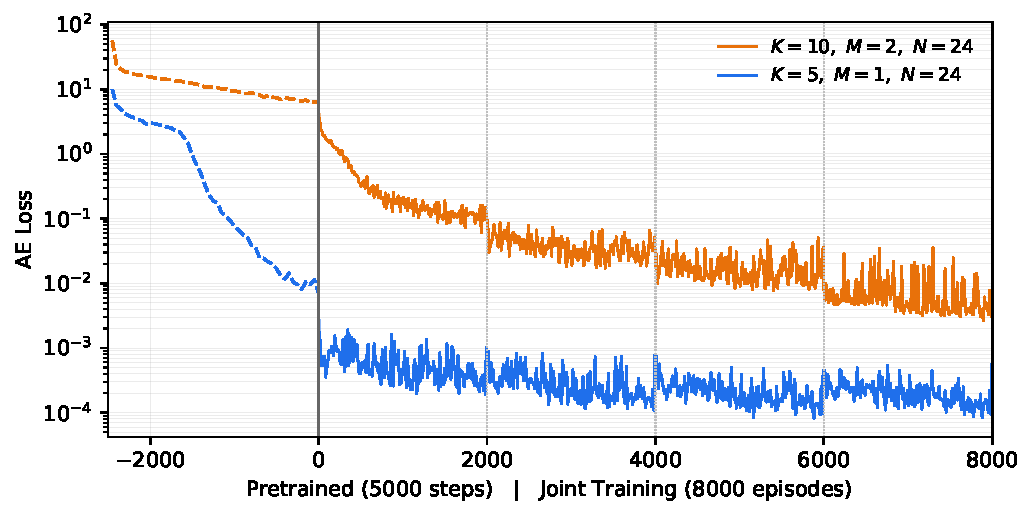
\includegraphics[width=\linewidth]{figures/ae_trajectory}
\caption{AE reconstruction loss $L_{AE}$ during autoencoder pre-training and subsequent joint RL training.}
\label{fig:ae_trajectory}
\end{figure}



% ---- A4 : VQC architectural choices -- user sẽ viết lại prose -------------
\subsection{VQC Architectural Choices}
\label{sec:abl_arch}
Five architectural choices define the quantum actor; each is varied one at a time against the reference configuration ($n_q{=}8$, $L{=}2$ and $L{=}3$ at the two scales, nearest-neighbor CZ chain with $M$ cross-block bridges, $R_yR_z$ angle encoding with data re-uploading, R1 readout).

\subsubsection{Circuit Depth}
The number of variational layers $L$ widens the accessible frequency spectrum of the re-uploading circuit~\cite{schuld2021effect}, so performance is expected to improve with $L$ up to saturation. The depth sweep is pending: \emph{---}.

\subsubsection{Entanglement Pattern}
Candidate patterns of increasing connectivity --- none, linear chain, ring, full --- are compared against the reference chain augmented with $M$ cross-block CZ bridges. The bridges are the problem-specific element: they couple the user- and IRS-qubit registers and are hypothesized to carry the user--IRS interaction that the assignment must model, whereas denser generic patterns add entanglement without this alignment. The toggle runs are pending: \emph{---}.

\subsubsection{Qubit Count and Latent Dimension}
The register size $n_q$ fixes the latent width $2n_q$ and hence the compression ratio $\bigl(K(M{+}2){+}2M\bigr)/2n_q$; it trades representation capacity against the $2^{n_q}$ simulation cost. The register is held at $n_q{=}8$ throughout; reducing it to six leaves performance inside the spread across training seeds (Section~\ref{sec:results_quantum}), and a wider sweep is pending: \emph{---}.

\subsubsection{Feature Map}
The reference encoding loads each latent pair through $R_y R_z$ rotations with a $\tanh$ squash and re-applies the encoding block at every layer (data re-uploading~\cite{perez2020data}). Alternative feature maps (amplitude encoding, IQP-style maps) change the accessible function class and the loading cost. A comparison is pending: \emph{---}.

\subsubsection{Readout Design}
The readout ladder varies the measured Pauli set at otherwise identical hyperparameters, from single-qubit $Z$ alone to sets that add two-qubit correlations of differing reach. The sets are not nested and their sizes do not rank them, so Table~\ref{tab:abl_readout} reports each case separately rather than as a monotone ladder.

\begin{table}[t]
\centering
\caption{Readout-design ablation, reported separately per case. All
configurations are identical except the measured observable set, and every
entry is a fresh run at $n_q{=}8$. $|\hat{\mathbf{o}}|$ is the number of
observables the policy layer receives. The R1 rows are the five-training-seed
main-table figures of Table~\ref{tab:case_main};
the ablation rows are single seeds and carry no spread. The cross-$ZZ$ set pairs every user qubit with every IRS qubit and adds nearest-neighbour pairs inside the user block; it is not the all-pairwise set, which would give $36$ observables at $n_q{=}8$. R1 carries one more observable than cross-$ZZ$ because it summarises each user's coupling to all other users in a single averaged term rather than in nearest-neighbour pairs, so $|\hat{\mathbf{o}}|$ does not order the sets by how much they measure.}
\label{tab:abl_readout}
% Filled 2026-08-20: Case-2 single-Z = r415/ep_00200, ONE seed.
%   Checkpoint by argmax return s.t. QoS>=90%% over all 6 checkpoints on
%   validation seeds 7/21/99 (reward 337.70, analysis/data/pick_r415.txt);
%   scored on test seeds 42/43/44 -> R_tot 1.7488 QoS 95.9%% reward 342.80
%   (analysis/data/tabXIII_c2_singlez_r415.txt).
%   For reference the Case-2 R1 row is the 5-seed main-table figure,
%   R_tot 1.742 +- 0.021 at QoS 94.4 +- 1.4%%, so single-Z with 8 observables
%   is inside the seed spread of R1 with 26.
% ⚠ The previous version of this table carried n_q=12 numbers (R1 = 34/42,
%   single-Z = 12/12) while the rest of the paper reports n_q=8, and it was not
%   marked stale. Every performance entry below therefore starts empty and is
%   filled only from an n_q=8 run.
% |o_hat| verified from the run logs (Post-NN input width minus n_latent=16):
%   single-Z 8/8, Z+NN-ZZ 15/15, Z+cross-ZZ 21/25, R1 22/26 (C1/C2).
%   R1 follows N_Q = (n_q - M)(M + 2) + M; confirmed at 26 on r289.
% Runs that fill each cell:
%   C1 single-Z r418 · C1 nn-ZZ r420 · C1 full-ZZ r421 · C1 R1 (main C1 VQC)
%   C2 single-Z r415 · C2 nn-ZZ r417 · C2 full-ZZ r419 · C2 R1 r289
\setlength{\tabcolsep}{4pt}
\begin{tabular}{lccc}
\toprule
Readout & Observables ($|\hat{\mathbf{o}}|$) & $R_{\mathrm{tot}}$ & QoS \\
\midrule
\multicolumn{4}{@{}l}{\emph{Case~1 ($K=5$, $M=1$)}} \\
\quad single-$Z$        & $8$  & \emph{---} & \emph{---} \\
\quad $Z$\,+\,NN-$ZZ$   & $15$ & \emph{---} & \emph{---} \\
\quad $Z$\,+\,cross-$ZZ$ & $21$ & \emph{---} & \emph{---} \\
\quad R1 (structured)   & $22$ & $2.482 \pm 0.100$ & $92.4 \pm 3.2\%$ \\
\midrule
\multicolumn{4}{@{}l}{\emph{Case~2 ($K=10$, $M=2$)}} \\
\quad single-$Z$        & $8$  & $1.749$ & $95.9\%$ \\
\quad $Z$\,+\,NN-$ZZ$   & $15$ & \emph{---} & \emph{---} \\
\quad $Z$\,+\,cross-$ZZ$ & $25$ & \emph{---} & \emph{---} \\
\quad R1 (structured)   & $26$ & $1.742 \pm 0.021$ & $94.4 \pm 1.4\%$ \\
\bottomrule
\end{tabular}
\end{table}

% ---- A5 : entropy regularization & annealing -- maps to C2 ----------------
\subsection{Entropy Regularization and Annealing}
\label{sec:abl_entropy}

% ---- A6 : power-fairness blending -- maps to the Power MLP execution path --
\fi

\end{document}